% Options for packages loaded elsewhere
% Options for packages loaded elsewhere
\PassOptionsToPackage{unicode}{hyperref}
\PassOptionsToPackage{hyphens}{url}
\PassOptionsToPackage{dvipsnames,svgnames,x11names}{xcolor}
%
\documentclass[
  referee]{gji}
\usepackage{xcolor}
\usepackage{amsmath,amssymb}
\setcounter{secnumdepth}{5}
\usepackage{iftex}
\ifPDFTeX
  \usepackage[T1]{fontenc}
  \usepackage[utf8]{inputenc}
  \usepackage{textcomp} % provide euro and other symbols
\else % if luatex or xetex
  \usepackage{unicode-math} % this also loads fontspec
  \defaultfontfeatures{Scale=MatchLowercase}
  \defaultfontfeatures[\rmfamily]{Ligatures=TeX,Scale=1}
\fi
\usepackage{lmodern}
\ifPDFTeX\else
  % xetex/luatex font selection
\fi
% Use upquote if available, for straight quotes in verbatim environments
\IfFileExists{upquote.sty}{\usepackage{upquote}}{}
\IfFileExists{microtype.sty}{% use microtype if available
  \usepackage[]{microtype}
  \UseMicrotypeSet[protrusion]{basicmath} % disable protrusion for tt fonts
}{}
\makeatletter
\@ifundefined{KOMAClassName}{% if non-KOMA class
  \IfFileExists{parskip.sty}{%
    \usepackage{parskip}
  }{% else
    \setlength{\parindent}{0pt}
    \setlength{\parskip}{6pt plus 2pt minus 1pt}}
}{% if KOMA class
  \KOMAoptions{parskip=half}}
\makeatother
% Make \paragraph and \subparagraph free-standing
\makeatletter
\ifx\paragraph\undefined\else
  \let\oldparagraph\paragraph
  \renewcommand{\paragraph}{
    \@ifstar
      \xxxParagraphStar
      \xxxParagraphNoStar
  }
  \newcommand{\xxxParagraphStar}[1]{\oldparagraph*{#1}\mbox{}}
  \newcommand{\xxxParagraphNoStar}[1]{\oldparagraph{#1}\mbox{}}
\fi
\ifx\subparagraph\undefined\else
  \let\oldsubparagraph\subparagraph
  \renewcommand{\subparagraph}{
    \@ifstar
      \xxxSubParagraphStar
      \xxxSubParagraphNoStar
  }
  \newcommand{\xxxSubParagraphStar}[1]{\oldsubparagraph*{#1}\mbox{}}
  \newcommand{\xxxSubParagraphNoStar}[1]{\oldsubparagraph{#1}\mbox{}}
\fi
\makeatother


\usepackage{longtable,booktabs,array}
\newcounter{none} % for unnumbered tables
\usepackage{calc} % for calculating minipage widths
% Correct order of tables after \paragraph or \subparagraph
\usepackage{etoolbox}
\makeatletter
\patchcmd\longtable{\par}{\if@noskipsec\mbox{}\fi\par}{}{}
\makeatother
% Allow footnotes in longtable head/foot
\IfFileExists{footnotehyper.sty}{\usepackage{footnotehyper}}{\usepackage{footnote}}
\makesavenoteenv{longtable}
\usepackage{graphicx}
\makeatletter
\newsavebox\pandoc@box
\newcommand*\pandocbounded[1]{% scales image to fit in text height/width
  \sbox\pandoc@box{#1}%
  \Gscale@div\@tempa{\textheight}{\dimexpr\ht\pandoc@box+\dp\pandoc@box\relax}%
  \Gscale@div\@tempb{\linewidth}{\wd\pandoc@box}%
  \ifdim\@tempb\p@<\@tempa\p@\let\@tempa\@tempb\fi% select the smaller of both
  \ifdim\@tempa\p@<\p@\scalebox{\@tempa}{\usebox\pandoc@box}%
  \else\usebox{\pandoc@box}%
  \fi%
}
% Set default figure placement to htbp
\def\fps@figure{htbp}
\makeatother





\setlength{\emergencystretch}{3em} % prevent overfull lines

\providecommand{\tightlist}{%
  \setlength{\itemsep}{0pt}\setlength{\parskip}{0pt}}




\usepackage[]{natbib}
\bibliographystyle{gji}


% Extra LaTeX loaded into the Quarto-rendered manuscript (paper/manuscript_marine.qmd).
% Quarto already provides geometry, graphicx, amsmath, hyperref, xcolor, longtable
% and booktabs; here we add only what the manuscript needs on top of that.

% gji.cls (a 1998-era class) hard-codes raw LaTeX-kernel tabular internals
% (\@tabclassz/\@tabclassiv/\@tabacol) in its \maketitle author-block macro,
% which the modern `array`/`tabularx` packages our tables depend on redefine --
% breaking \maketitle with "Missing # inserted in alignment preamble" right
% after the title block (confirmed by isolated bisection: `array` alone
% reproduces it). gji-siunitx-patch.sty is GJI's own official 2019 patch
% (shipped in their Overleaf template, originally written to fix a siunitx
% clash) that replaces \@maketitle/\author/\and with plain, non-tabular
% versions -- which also happens to remove the exact mechanism that conflicts
% with array/tabularx. Load it right after \documentclass{gji}.
\usepackage{gji-siunitx-patch}

% gji.cls only defines \newblock *inside* its own \thebibliography macro, but
% natbib (loaded via cite-method: natbib) redefines \thebibliography wholesale
% for author-year/numeric switching -- so gji.cls's inline definition never
% runs, and the natbib-generated .bbl calls an undefined \newblock. Provide it
% standalone with the class's own spacing (the standard fix for classes that
% never define \newblock as a top-level command).
\providecommand{\newblock}{\hskip .11em plus .33em minus .07em}

\usepackage{siunitx}
\usepackage{tabularx}
\usepackage{array}
\usepackage{booktabs}
\newcolumntype{L}{>{\raggedright\arraybackslash}X}

% Let floats pack densely so the in-text tables land near their reference and do
% not collide with the bibliography; the big survey table is a longtable (flows).
\renewcommand{\topfraction}{0.92}
\renewcommand{\bottomfraction}{0.85}
\renewcommand{\textfraction}{0.07}
\renewcommand{\floatpagefraction}{0.72}
\setcounter{topnumber}{3}
\setcounter{totalnumber}{4}

% Figures live in the survey's figure directory.
\graphicspath{{../literature/figs/}{figs/}}

\providecommand{\dvv}{\ensuremath{\delta v/v}}

% --- GJI (Geophysical Journal International) formatting ----------------------
% gji.cls redefines \abstract/\endabstract to its own \summary environment
% (which hardcodes the "SUMMARY" heading itself, not via \abstractname -- the
% class does not define \abstractname at all), so nothing else is needed here
% for the summary heading. Key words are set via the raw
% ```{=latex}\keywords ... \endkeywords``` block in the manuscript body.

% Continuous line numbers, patched to survive amsmath display environments.
\usepackage{lineno}
\newcommand*\patchAmsForLineno[1]{%
  \expandafter\let\csname old#1\expandafter\endcsname\csname #1\endcsname
  \expandafter\let\csname oldend#1\expandafter\endcsname\csname end#1\endcsname
  \renewenvironment{#1}%
    {\linenomath\csname old#1\endcsname}%
    {\csname oldend#1\endcsname\endlinenomath}}%
\newcommand*\patchBothAmsForLineno[1]{\patchAmsForLineno{#1}\patchAmsForLineno{#1*}}%
\AtBeginDocument{%
  \patchBothAmsForLineno{equation}%
  \patchBothAmsForLineno{align}%
  \patchBothAmsForLineno{gather}%
  \patchBothAmsForLineno{multline}%
  \patchBothAmsForLineno{flalign}%
  \patchBothAmsForLineno{alignat}%
}
\linenumbers

% Double-spaced text (GJI review), tables kept single-spaced for legibility.
% \doublespacing itself looks up a per-pointsize stretch table via \@ptsize, a
% standard-class counter gji.cls (an old, non-standard LaTeX2e class) never
% defines; \setstretch{2} sets the same 2x line stretch directly, with no
% \@ptsize dependency.
\usepackage{setspace}
\setstretch{2}
\usepackage{etoolbox}
\AtBeginEnvironment{tabular}{\singlespacing}
\AtBeginEnvironment{tabularx}{\singlespacing}
\AtBeginEnvironment{longtable}{\singlespacing}
\makeatletter
\@ifpackageloaded{caption}{}{\usepackage{caption}}
\AtBeginDocument{%
\ifdefined\contentsname
  \renewcommand*\contentsname{Table of contents}
\else
  \newcommand\contentsname{Table of contents}
\fi
\ifdefined\listfigurename
  \renewcommand*\listfigurename{List of Figures}
\else
  \newcommand\listfigurename{List of Figures}
\fi
\ifdefined\listtablename
  \renewcommand*\listtablename{List of Tables}
\else
  \newcommand\listtablename{List of Tables}
\fi
\ifdefined\figurename
  \renewcommand*\figurename{Figure}
\else
  \newcommand\figurename{Figure}
\fi
\ifdefined\tablename
  \renewcommand*\tablename{Table}
\else
  \newcommand\tablename{Table}
\fi
}
\@ifpackageloaded{float}{}{\usepackage{float}}
\floatstyle{ruled}
\@ifundefined{c@chapter}{\newfloat{codelisting}{h}{lop}}{\newfloat{codelisting}{h}{lop}[chapter]}
\floatname{codelisting}{Listing}
\newcommand*\listoflistings{\listof{codelisting}{List of Listings}}
\makeatother
\makeatletter
\makeatother
\makeatletter
\@ifpackageloaded{caption}{}{\usepackage{caption}}
\@ifpackageloaded{subcaption}{}{\usepackage{subcaption}}
\makeatother
\usepackage{bookmark}
\IfFileExists{xurl.sty}{\usepackage{xurl}}{} % add URL line breaks if available
\urlstyle{same}
\hypersetup{
  pdftitle={The reproducibility cost of ad-hoc processing choices in ambient-noise seismic velocity-change monitoring},
  pdfauthor={M. A. Denolle},
  colorlinks=true,
  linkcolor={blue},
  filecolor={Maroon},
  citecolor={Blue},
  urlcolor={Blue},
  pdfcreator={LaTeX via pandoc}}


\title{The reproducibility cost of ad-hoc processing choices in
ambient-noise seismic velocity-change monitoring}
\author{M. A. Denolle}
\date{2026-07-22}
\begin{document}
\maketitle
\begin{abstract}
Relative seismic velocity changes (\dvv) from the ambient seismic field
are a standard observable for volcanoes, faults, landslides, aquifers
and the cryosphere. Yet turning cross-correlation functions into a
\dvv~time series involves a long sequence of choices --- the estimator,
the frequency band, the coda window, the reference, the stacking, and
how cross-components and station pairs are aggregated and weighted ---
made \emph{ad hoc} and seldom reported in full. Using a controlled
synthetic in which the ground-truth \dvv~is known exactly, we quantify
how much each choice moves the recovered value \emph{and its stated
uncertainty}. Reproducing the seven NoisePy estimators, we show that at
large \dvv~methods split by family with distinct failure modes; that the
same station pair yields different \dvv~depending only on whether one
averages the per-component \dvv~or the correlation-coefficient images;
and, most consequentially, that the reported \(1\sigma\) on a
network-averaged \dvv~varies by \(\sim\!\sqrt{N}\) from the
standard-error-versus-standard-deviation and weighting conventions ---
so a change that is ``\(3\sigma\) significant'' in one study is ``not
significant'' in another, from identical data. Running the full
\emph{multiverse} of choices, we rank each by the bias and error-bar
change it induces, and propose a Bayesian measurement model that
marginalises the ensemble into a single time-dependent data covariance
\(C_d\) --- the object a downstream depth or stress inversion needs. We
argue that these undocumented choices, not the physics, are the leading
obstacle to intercomparing \dvv~studies, and release an open framework
(codameter) that makes every choice explicit and reproducible.
\end{abstract}


\begin{keywords}
Time-series analysis; Interferometry; Seismic noise; Coda waves; Inverse theory; Statistical methods.
\end{keywords}

\section{Introduction}\label{sec:intro}

Changes in subsurface properties occur due geodynamics, which drive
earthquake damage and volcanic eruption, and hydrodynamics, which
controls fluid exchange between the atomsphere and the solid Earth.
These processes influence the mechanical property of Earth materials,
which directly affect the speed at which seismic waves propagates.
Changes in seismic velocity, often measured and referred to as \dvv, can
be tracked by measuring changes in arrival times of seismic waves,
especially scatterd waves such as coda waves, provided that the source
and receivers are at the same location.

Due to the sensitivity of coda waves to small perturbations in the
material properties, \dvv~was discovered as an effective method to
monitor chanes during volcanic unrest since its discovery at Piton de la
Fournaise \citep{Brenguier2008} and is now calculated in continuous
along side of more conventional seismic monitoring methods in the same
volcano observatory \citep{Duputel2009} and was a determining early
warning parameter used by the Icelandic Meteorological Office used
\dvv~in its response to the 2020 Reykjanes unrest (Cubuk-Sabuncu et al.,
2021). The Institute of Mine Seismology also uses \dvv~to monitor the
internal state of tens of tailings dams and mines to flag instability
before failure (Olivier et al., 2017; Ouellet et al., 2022). A broader
set of operations is emerging around the same signal: groundwater
storage for water management (Clements and Denolle, 2018; Mao et al.,
2022), landslide early warning (Le Breton et al., 2021), levee and
embankment integrity (Planès et al., 2016), and geothermal and CO\(_2\)
reservoir surveillance (Nakata et al., 2021). Each of these deployments
rests on the same fragile assumption: that the \dvv~curve an operator
acts on is a property of the subsurface, not of the analyst's processing
choices.

The elevated sensitivity comes at the price a long series of processing
choices and at almost every step the analyst makes a choice. Among these
are choices of estimators between windowed phase measurements or
strething \citep[\citet{Mao2020}, \citet{Yuan2021}]{Mikesell2015},
frequency band and coda window (which together set the sampled depth;
\citeauthor{Obermann2013}
\citetext{\citeyear{Obermann2013}; \citealp{Obermann2016}}), reference
window \citep[\citet{Ermert2023}, \citet{Okubo24}]{Brenguier2014}, how
much to substack to increase coherence among windows (Hadzianou Celine),
and how to aggregate and weight the many cross-component and
station-pair measurements that make up a single reported \dvv~time
series (e.g., \citet{hobiger14}). These choices are typically made by
habit, justified briefly if at all , and rarely reported in enough
detail to reproduce. The community has long flagged \emph{individual}
pitfalls (spurious changes from non-stationary noise, \citet{Zhan2013};
measurement-error formulae, \citeauthor{Clarke2011}
\citetext{\citeyear{Clarke2011}; \citealp{Weaver2011}}), but the
\emph{cumulative} effect of the full choice set on both the value and
its stated uncertainty has not been quantified comprehensively in the
literature.

This is a reproducibility problem of exactly the ``garden of forking
paths'' type identified in the statistical sciences
\citep{Gelman2013, Steegen2016}: many individually reasonable analyses
of the same data give different answers, and without full reporting
parameter choices we cannot fully interpret \dvv~as robust values. .
Here we make the problem concrete for \dvv~monitoring. We use purely
synthetic correlation time series to test the methods (estimators) and
parameter choices that the community makes to estimate \dvv, which we
report over 103 studies Appendix\textasciitilde{}\ref{app:survey}. We do
not aim to report the ``best'' pipeline, which is most often the one
reported in scientific papers, but instead document the various
parameter impacts (Section\textasciitilde{}\ref{sec:results}). We then
propose a new measurement error that incoporates these effects into a
data covariance matrix \(C_d\)
(Section\textasciitilde{}\ref{sec:bayes}).

One example of propagating such error in downstream scientific insights
is the migration of the surface \dvv~measurement to depth profiles of
perturbations in shear wave velocity \(\Delta V_S(z)/V_S(z)\), which
often depends on the wavefield constituting the coda waves, such as
surface waves or body waves, and that depend on the source-receiver pair
geometry. We illustrate the propagation of errors to a depth profile
(Section\textasciitilde{}\ref{sec:depth}). We only utilize synthetic
examples for ground truthing on the signal processing parameters, since
the concepts behind the observations of phase lags in scattered waves is
well established \citep{Obermann2013}. We package this new methodology
in a Python software, \texttt{codameter}, which we also recast as an
agentic system with skill, examples of golden data sets, and its
evaluation against base models.

\section{Synthetic framework}\label{sec:methods}

We build each synthetic reference coda wave as a band-limited
random-phase wavefield modulated by a physically grounded coda envelope.
We model the envelope from the exact single-scattering solution of the
two-dimensional radiative transfer equation for isotropic scattering
\citep{Sato1993, Paasschens1997}, which underlies coda-envelope
modelling of scattering and intrinsic attenuation \citep{Margerin1998}.
The energy density at source--receiver distance \(r\) and lapse time
\(t\) is

\begin{linenomath*}
\begin{equation}
E(r,t)=\left[\frac{e^{-ct/\ell}}{2\pi c r}\,\delta\!\left(t-\frac{r}{c}\right) +
\frac{e^{\frac{1}{\ell}\left(\sqrt{c^2 t^2-r^2}-ct\right)}}{2\pi \ell\sqrt{c^2 t^2-r^2}}\,
H\!\left(t-\frac{r}{c}\right)\right] e^{-b t},
\label{eq:rt2d}
\end{equation}
\end{linenomath*}

where \(c\) is the (Rayleigh-wave) velocity, \(\ell\) the scattering
mean free path, \(b\) the intrinsic absorption rate, and \(\delta\) and
\(H\) the Dirac and Heaviside functions. The first term is the coherent
ballistic arrival at \(t=r/c\); the second is the multiply-scattered
diffuse coda, which switches on at that arrival, builds up under
scattering, and decays under intrinsic absorption. We fill random phases
under the amplitude envelope \(\sqrt{E(r,t)}\), band-limit, and
symmetrize the causal and acausal branches as for an evenly illuminated
noise correlation. The modeled synthetic coda depends only on three time
constants: the ballistic onset \(r/c\), the scattering mean free time
\(\ell/c\), and the absorption time \(1/b\). The late-coda amplitude
decays as \(e^{-b t/2}\), recovering an apparent coda \(Q_c\) while the
envelope \emph{shape} is determined by scattering physics. A
frequency-dependent absorption \(b(f)=2\pi f/Q_c\), which can still be
modeled as an frequency-independent attenuation factor \(Q_c\),
reproduces the observation that high frequencies are retained only at
short lag times, so a fixed late window samples different depths at
different bands.

A homogeneous velocity change is imposed exactly by stretching the
lapse-time axis,
\(u_{\rm cur}(t) = u_{\rm ref}\!\left(t/(1+\dvv)\right)\), and a
repeated time series is produced by generating this stretched coda with
a prescribed ground-truth \(\dvv(t)\) and additive band-limited noise at
a controlled signal-to-noise ratio. The concept has been demonstrated
using full waveform modeling in several previous studies
(\citet{Obermann2013}, \citet{Obermann2016},\citet{Yuan2021}), therefore
we do not model these effects using full waveforms. Because the imposed
\(\dvv(t)\) is known, every departure of a recovered series from it is
an artefact of the processing, not of the data.

We utilize seven \dvv~estimators that were implemented in
\texttt{noisepy} in the \texttt{monitoring\_methods} module
\citep{Jiang2020}: trace stretching (TS, \citet{lobkis01}), windowed
cross-correlation (WCC, \citet{poupinet84}), dynamic time warping (DTW,
\citet{Mikesell2015}), te moving-window cross-spectrum (MWCS;
\citet{Clarke2011}), and three wavelet-domain methods, the wavelet
cross-spectrum (WCS, \citet{Mao2020}) and the two wavelet stretching
(WTS) and wavelet DTW (WTDTW) introduced and benchmarked numerically by
\citet{Yuan2021}. The framework, the figures below, and a implementation
are released in the open \texttt{codameter} package
(Section\textasciitilde{}\ref{sec:discussion}). Formal definitions of
all seven methods, of the two aggregation pathways, and of the
uncertainty conventions are described in
Appendices\textasciitilde{}\ref{app:estimators}
and\textasciitilde{}\ref{app:aggregation}.

Each of these methods require specific parameter choices, which we
categorize and reference in Table\textasciitilde{}\ref{tab:hyperparams}.
The work presented below measure the impacts of each of these parameter
choices on the resulting \dvv.

\begin{table}
\footnotesize
\caption{Processing choices (``hyper-parameters'') and their effect on the
recovered value and the reported uncertainty ($B$: bandwidth, $N$: measurement
count, $N_{\mathrm{eff}}$: weighted effective count).}
\label{tab:hyperparams}
\begin{tabularx}{\textwidth}{@{}>{\raggedright\arraybackslash}p{2.35cm} L L L@{}}
\toprule
\textbf{Choice} & \textbf{Options / typical range} & \textbf{Effect on the
value} & \textbf{Effect on the uncertainty} \\
\midrule
Estimator & TS, WCC, DTW, MWCS, WCS, WTS, WTDTW (7 in NoisePy) &
Agree at small \dvv; at large \dvv\ phase methods cycle-skip, warps under-shoot
(Fig.~\ref{fig:methods}) & Each has its own error model; the inter-method spread
is itself an uncertainty \\ \hline
Phase unwrapping & on / off (phase methods) & Decides whether MWCS/WCS cycle-skip
(Fig.~\ref{fig:methods}b) & Sets the usable \dvv\ range \\ \hline
Frequency band $[f_1,f_2]$ & 0.1--2\,Hz (volcano), 2--4\,Hz (aquifer),
4--12\,Hz (landslide) & Selects the sampled depth, hence \emph{which} signal
(Fig.~\ref{fig:params}a) & $\sigma$ falls as bandwidth $B$ grows \\ \hline
Coda window $[t_1,t_2]$ & a few to tens of mean free times & Later lapse $\to$
deeper, larger sensitivity & $\sigma\propto(t_2^3-t_1^3)^{-1/2}$, but late coda
is low-SNR \\ \hline
Window--band coupling & fixed vs scaled with $f$ & A fixed late window at high
$f$ measures noise (Fig.~\ref{fig:params}b) & Inflates $\sigma$ / decorrelation
at high band \\ \hline
Reference & total stack / trailing / joint inversion & Moving reference erases
slow trends (Fig.~\ref{fig:params}c) & Reference noise propagates; inversion
lowers it \\ \hline
Stacking / substack & 1--30+ days & Smears and delays transients
(Fig.~\ref{fig:params}d) & $\sigma$ falls with stack length; resolution falls
too \\ \hline
Component aggregation & A (average \dvv) vs B (average CC images); weighted vs
not & Different time series (Fig.~\ref{fig:aggregation}) & Different uncertainty
object (ensemble spread vs CC-peak width) \\ \hline
Pair / network weighting & coherence-weighted vs unweighted & Small change in
value & Changes $N_{\mathrm{eff}}$ \\ \hline
Uncertainty definition & within-measurement (Weaver) / SE / SD &
--- & Factor $\sqrt{N}$ or more (Fig.~\ref{fig:uncertainty}) \\ \hline
Quality control & min CC, min SNR, max $\delta t$ error & Rejects or keeps
measurements & Sets the effective $N$ and any selection bias \\ \hline
Pre-processing & one-bit / running-mean; whitening band & Bias if the noise
field is non-stationary & Spurious \dvv\ when the noise spectrum drifts
\citep{Zhan2013} \\ \hline
Clock / timing & causal vs acausal branch handling & A clock error fabricates
\dvv\ (Fig.~\ref{fig:artifacts}a) & Branch asymmetry diagnoses it \\
\bottomrule
\end{tabularx}
\end{table}

\section{Measurement: how the choices move the velocity change and its
error}\label{sec:results}

The literature agrees on the components of a well-posed \dvv~measurement
--- a stretching-family estimator for robustness at low SNR and large
change \citep{Mikesell2015, Yuan2021}, a coherence-based error model
\citep{Clarke2011, Weaver2011}, a long stable reference
\citep{Wang2017}, and cross-validation against a second estimator
\citep{Obermann2019} --- yet studies do not always report the same set,
and the uncertainty convention is rarely, if ever, quantified
(Appendix\textasciitilde{}\ref{app:survey}). The sections below address
each component in turn and quantify, against a known truth, how far a
reasonable deviation moves the recovered value and its stated error. The
deliverable of this section is a measurement covariance, which every
subsequent step in the inference chain
(Sections\textasciitilde{}\ref{sec:depth}--\ref{sec:stress}) consumes.

\subsection{Estimator family}\label{sec:methods-fig}

\subsection{TO REVIEW}\label{to-review}

On small, clean \dvv, all seven estimators agree, demonstrating
robustness of the methods (Fig.\textasciitilde{}\ref{fig:methods}a). The
estimator choice becomes consequential at large
\dvv~(Fig.\textasciitilde{}\ref{fig:methods}b), where the methods split
by family. The stretching family (TS, WTS) and WCC match the whole
dilated coda and remain accurate; the phase methods read a wrapped
phase, so MWCS cycle-skips, while the \emph{same} cross-wavelet phase,
once unwrapped in 2-D, recovers the change --- success or failure
turning on the unwrapping sub-choice alone. The warping methods (DTW,
WTDTW) track but under-shoot the largest strains. No estimator is simply
``right''; an undocumented estimator choice can alters the
\dvv~measurements for larger strain changes.

The wavelet methods use a dependency-free Morlet continuous wavelet
transform; WCS optionally unwraps the cross-wavelet phase in two
dimensions (along lapse, anchored at \(\tau\!\to\!0\), then along
frequency) following \citet{Mao2020}.

\begin{figure}
  \centering
  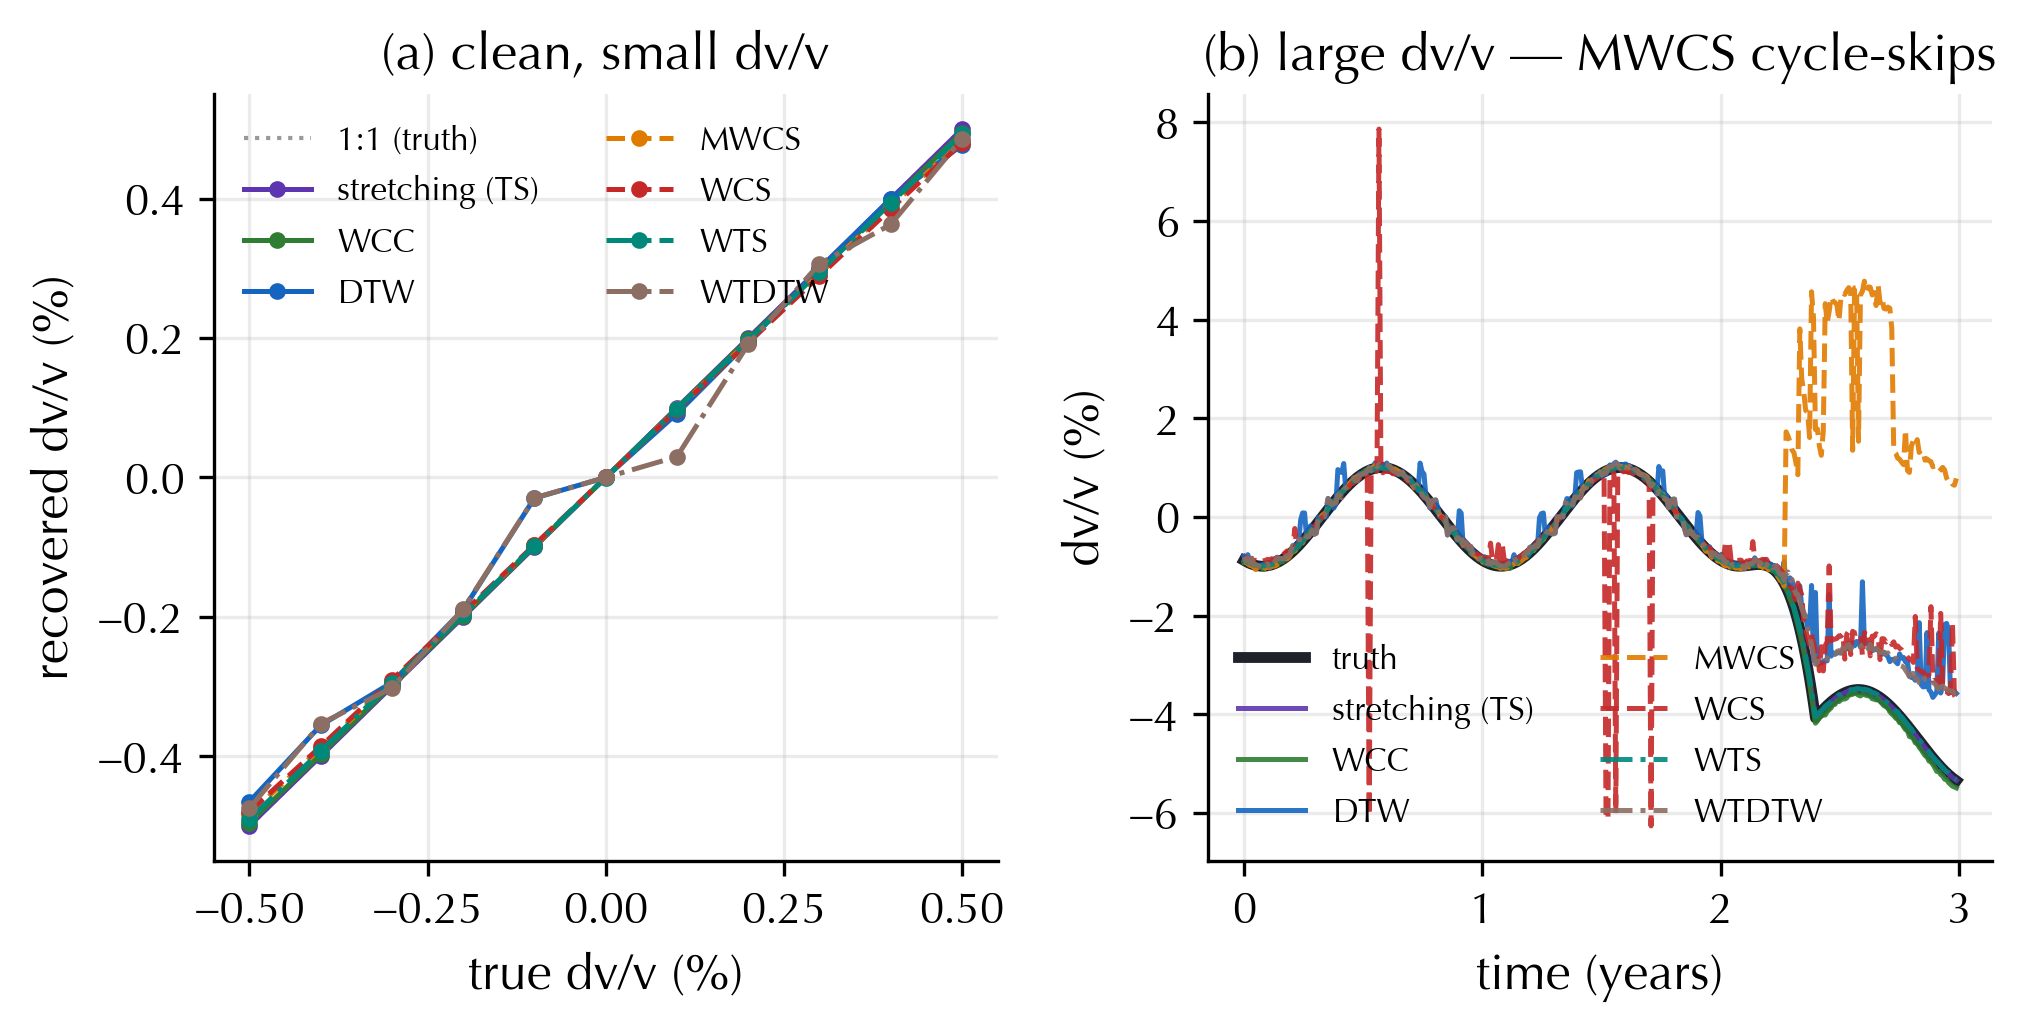
\includegraphics[width=\textwidth]{demo_1_methods.png}
  \caption{Estimator choice across the seven NoisePy methods. (a) Clean,
  small \dvv: all agree. (b) Large \dvv\ (a pre-failure landslide signal): MWCS
  cycle-skips, 2-D-unwrapped WCS and the stretching family track, the warping
  methods under-shoot.}
  \label{fig:methods}
\end{figure}

\subsection{Aggregating cross-components}\label{sec:aggregation}

Each three-component seismic station (e.g., Z, N, E) carries 6
cross-componet correlations (ZZ, NN, EE, ZE, ZN, NE), whether they are
calculated at the single station or a inter-station pair. Each carry a
signature of the changes in velocity, components may be dominated by
Love or Rayleigh waves (REF), but there scattering and non-straight ray
path induce cross-component leakage between modes (REF), and thus it is
often assumed in practice that coda waves of cross-components with
multi-scattering characteristixcs (e.g., no clearly separated phases)
are compoed of ``surface waves'' with strong S-wave sensitivity.
Combining them together requires parameter choices, such as averaging
them directly (REF), or weighted (e.g., using coherence-based weighting
\citet{hobiger14}). Combining is another workflow choice that can change
both the value and the uncertainty
(Fig.\textasciitilde{}\ref{fig:aggregation}). One may peak-pick each
component's correlation-coefficient curve \(\mathrm{CC}(\varepsilon,t)\)
and then average the per-component \dvv~(Approach A) --- unweighted, a
few poor components bias the mean; coherence-weighted, they are
suppressed --- or one may average the \(\mathrm{CC}(\varepsilon,t)\)
\emph{images} across components first and peak-pick once (Approach B).
All three conventions appear in the literature; on the same pair they
give visibly different time series, and they propagate uncertainty along
incompatible pathways (the ensemble spread of the per-component picks
for A, the width of the averaged correlation peak for B).

\begin{figure}
  \centering
  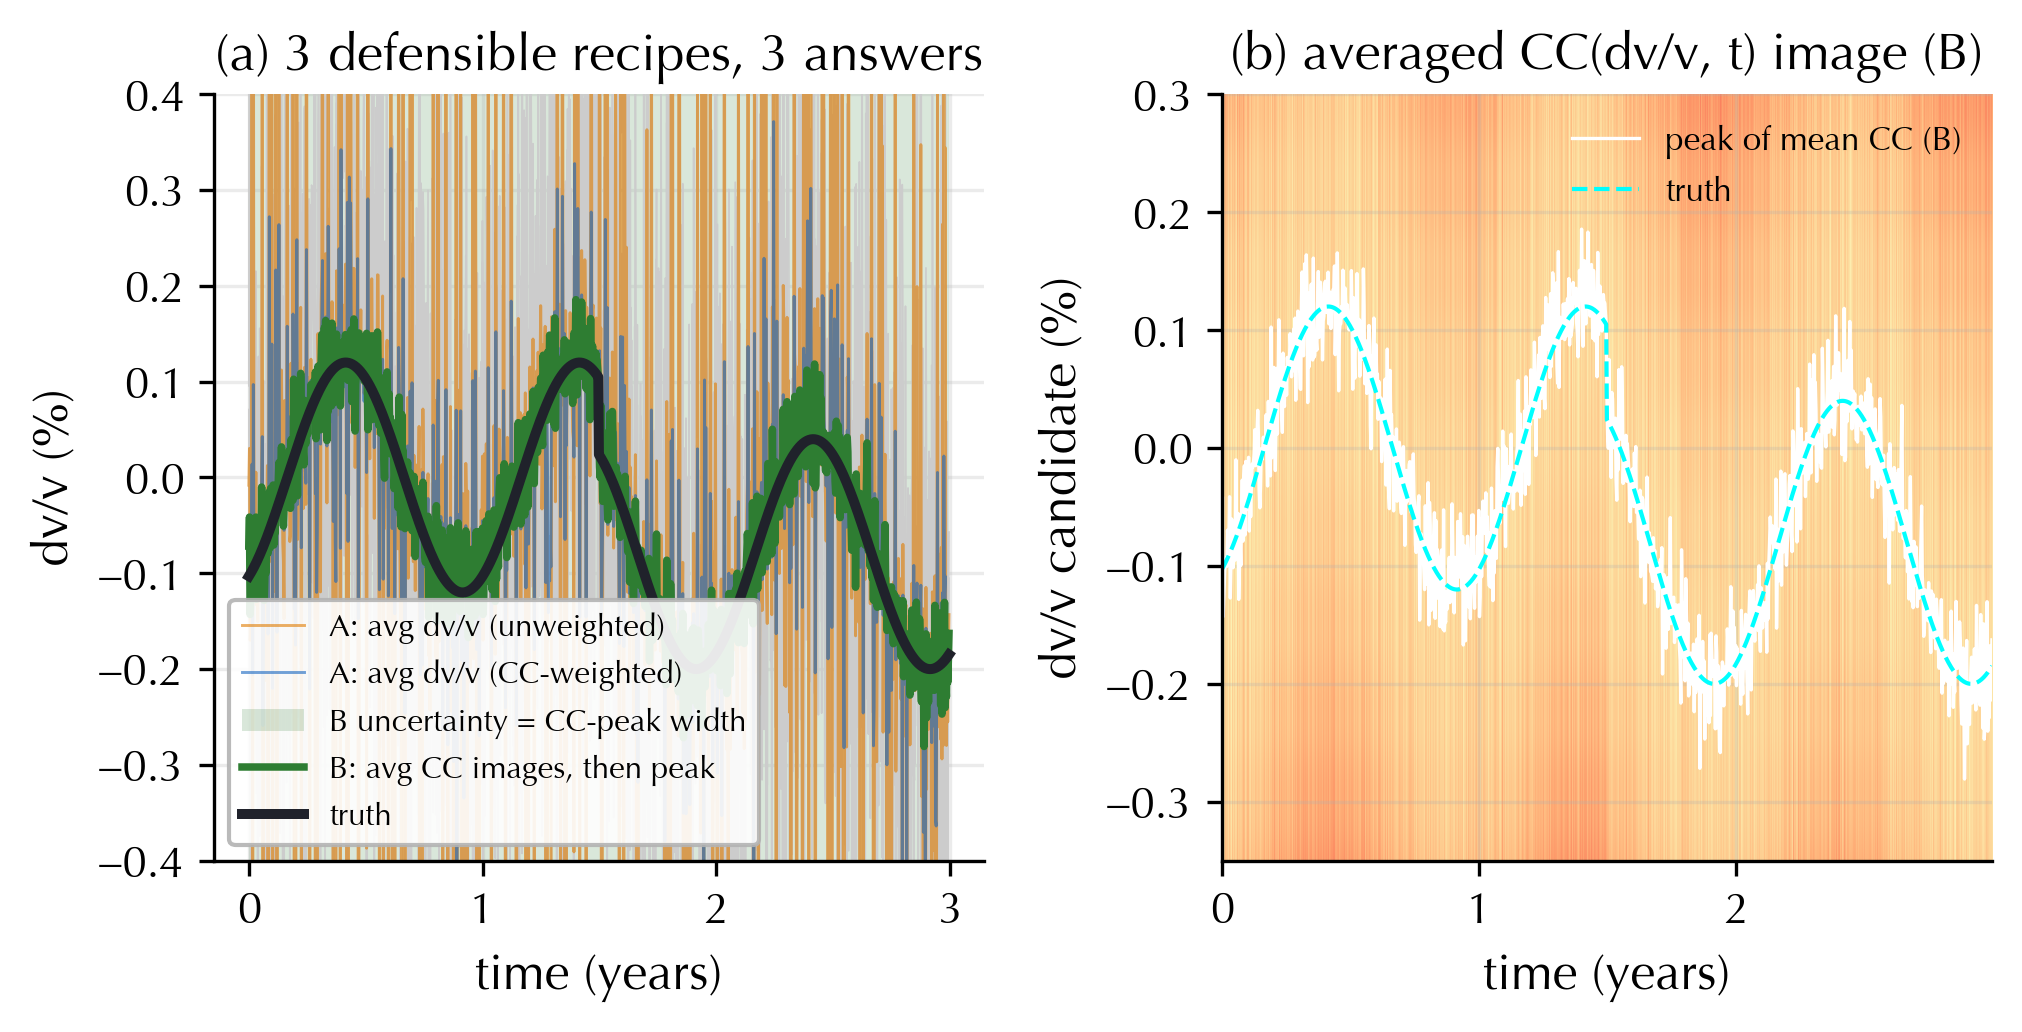
\includegraphics[width=\textwidth]{demo_2_aggregation.png}
  \caption{Cross-component aggregation for one station pair. (a) Unweighted
  \dvv-averaging is biased by the poor components, while coherence-weighting and
  image-averaging track the truth. (b) The averaged $\mathrm{CC}(\dvv,t)$ image
  of Approach B with its peak ridge.}
  \label{fig:aggregation}
\end{figure}

\subsection{Network aggregation and the reported error
bar}\label{sec:uncertainty}

Adding the next layer up --- combining many station pairs into a network
series --- exposes the most consequential and least-reported choice of
all: how to summarize the uncertainty. Three conventions are common: a
coherence-weighted standard error, an unweighted standard error
(\(\sigma=\mathrm{std}/\sqrt{N}\)), and the between-pair standard
deviation (the scatter, \emph{not} divided by \(\sqrt{N}\)). On the same
synthetic network the recovered means nearly coincide, but the reported
\(1\sigma\) spans a factor of \(\sim\!\sqrt{N}\)
(Fig.\textasciitilde{}\ref{fig:uncertainty}). A velocity change that is
``\(3\sigma\) significant'' under the tightest convention is
``\(1\sigma\), not significant'' under the most conservative one ---
from identical data. Error bars on published \dvv~are therefore not
comparable across studies unless the aggregation, the weighting, and the
standard-error-versus-standard-deviation convention are all stated.

\begin{figure}
  \centering
  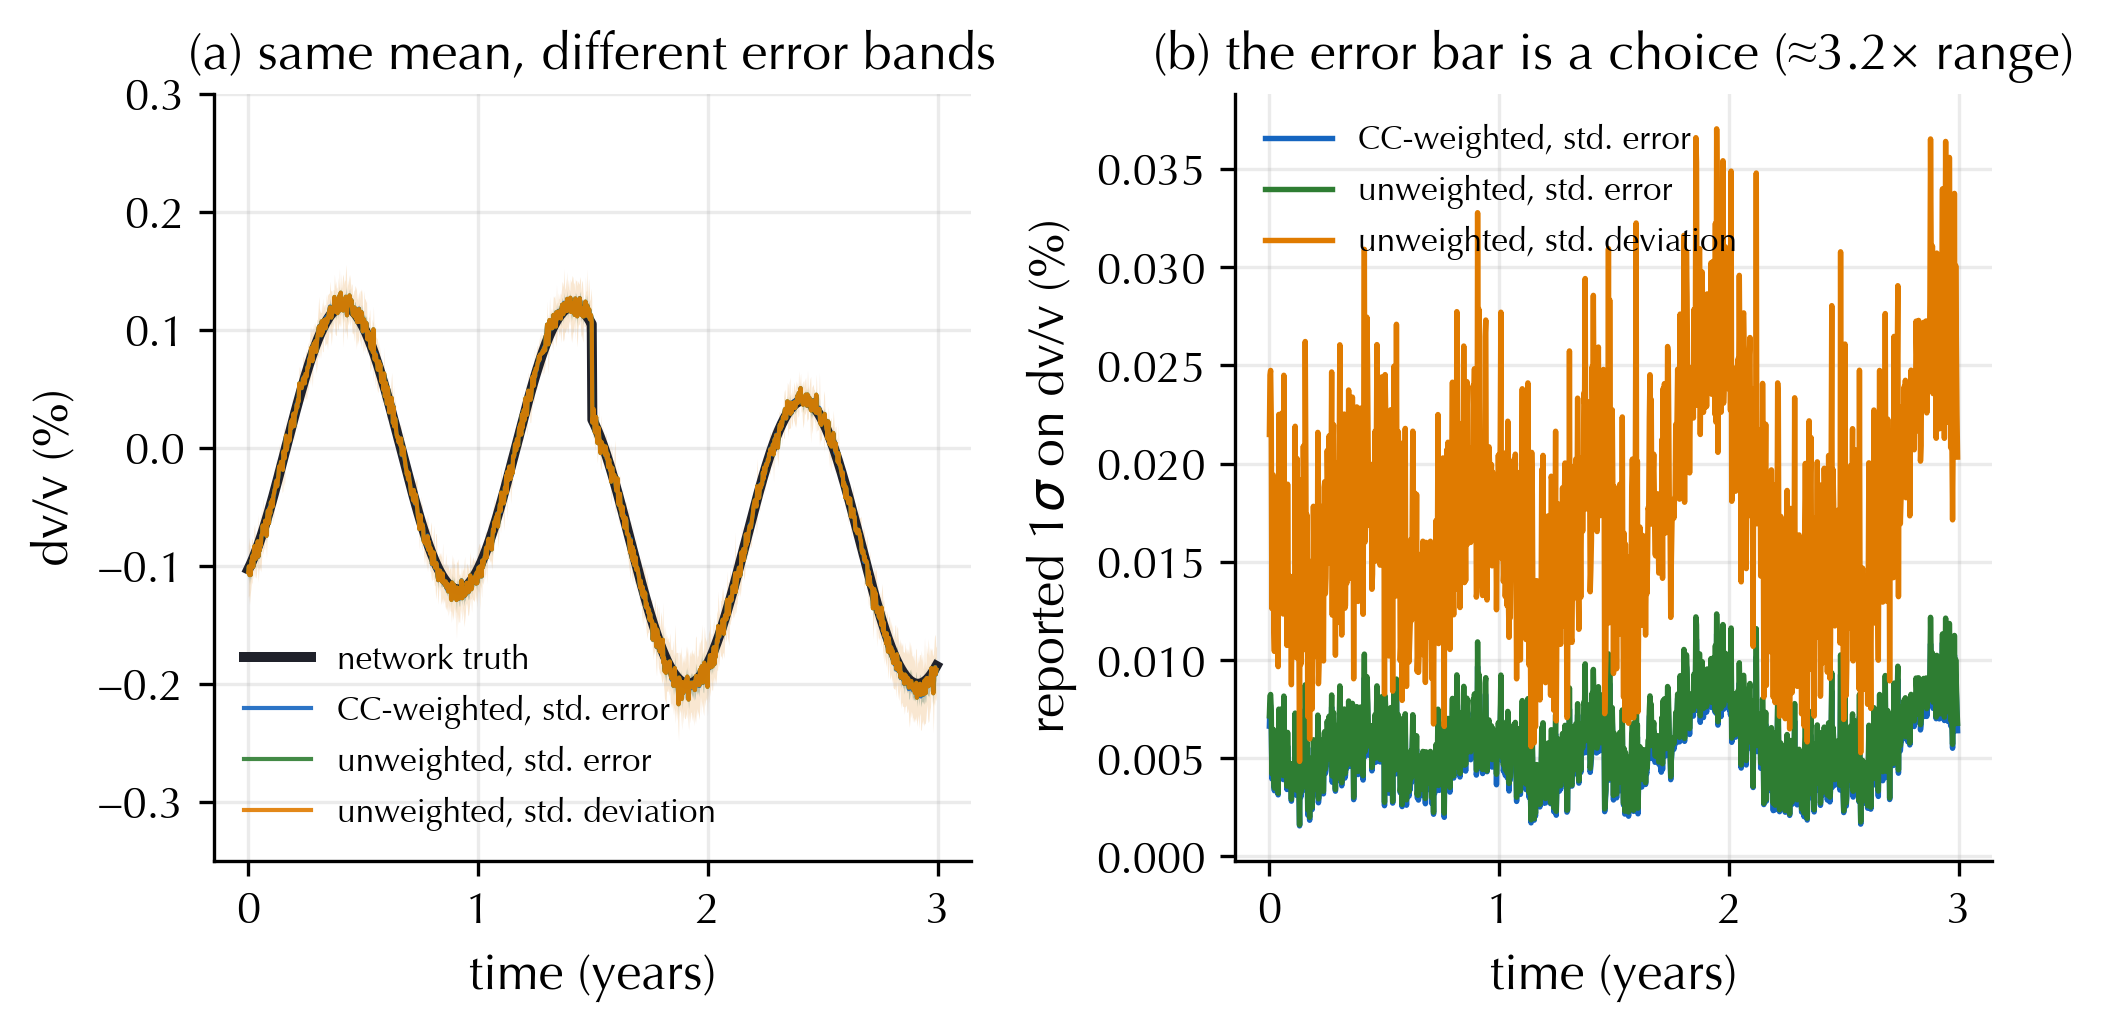
\includegraphics[width=\textwidth]{demo_3_uncertainty.png}
  \caption{Station-pair aggregation and uncertainty for a nine-pair network. (a)
  The recovered \dvv\ agrees across conventions; the shaded $1\sigma$ bands do
  not. (b) The reported $1\sigma$ differs by $\sim\!\sqrt{N}$ purely from the
  weighting and SE-versus-SD choices.}
  \label{fig:uncertainty}
\end{figure}

\subsection{Frequency band, coda window, reference and
stacking}\label{sec:params}

The remaining choices are no less consequential. The frequency band sets
the sampled depth: in a two-layer medium, banding high recovers a
shallow seasonal signal and banding low recovers a deep trend --- the
band chooses \emph{what is measured}
(Fig.\textasciitilde{}\ref{fig:params}a). The coda window does not
transfer across bands: because the coda fades first at high frequency, a
late window that is full of signal at low frequency is pure noise at
high frequency, and reusing it recovers only noise
(Fig.\textasciitilde{}\ref{fig:params}b). The reference defines what
survives: a moving reference re-baselines continuously and erases slow
trends that a fixed reference or a joint inversion \citep{Brenguier2014}
preserve (Fig.\textasciitilde{}\ref{fig:params}c). And the stacking
length trades noise against temporal resolution, rounding off and
delaying a coseismic step (Fig.\textasciitilde{}\ref{fig:params}d).

\begin{figure}
  \centering
  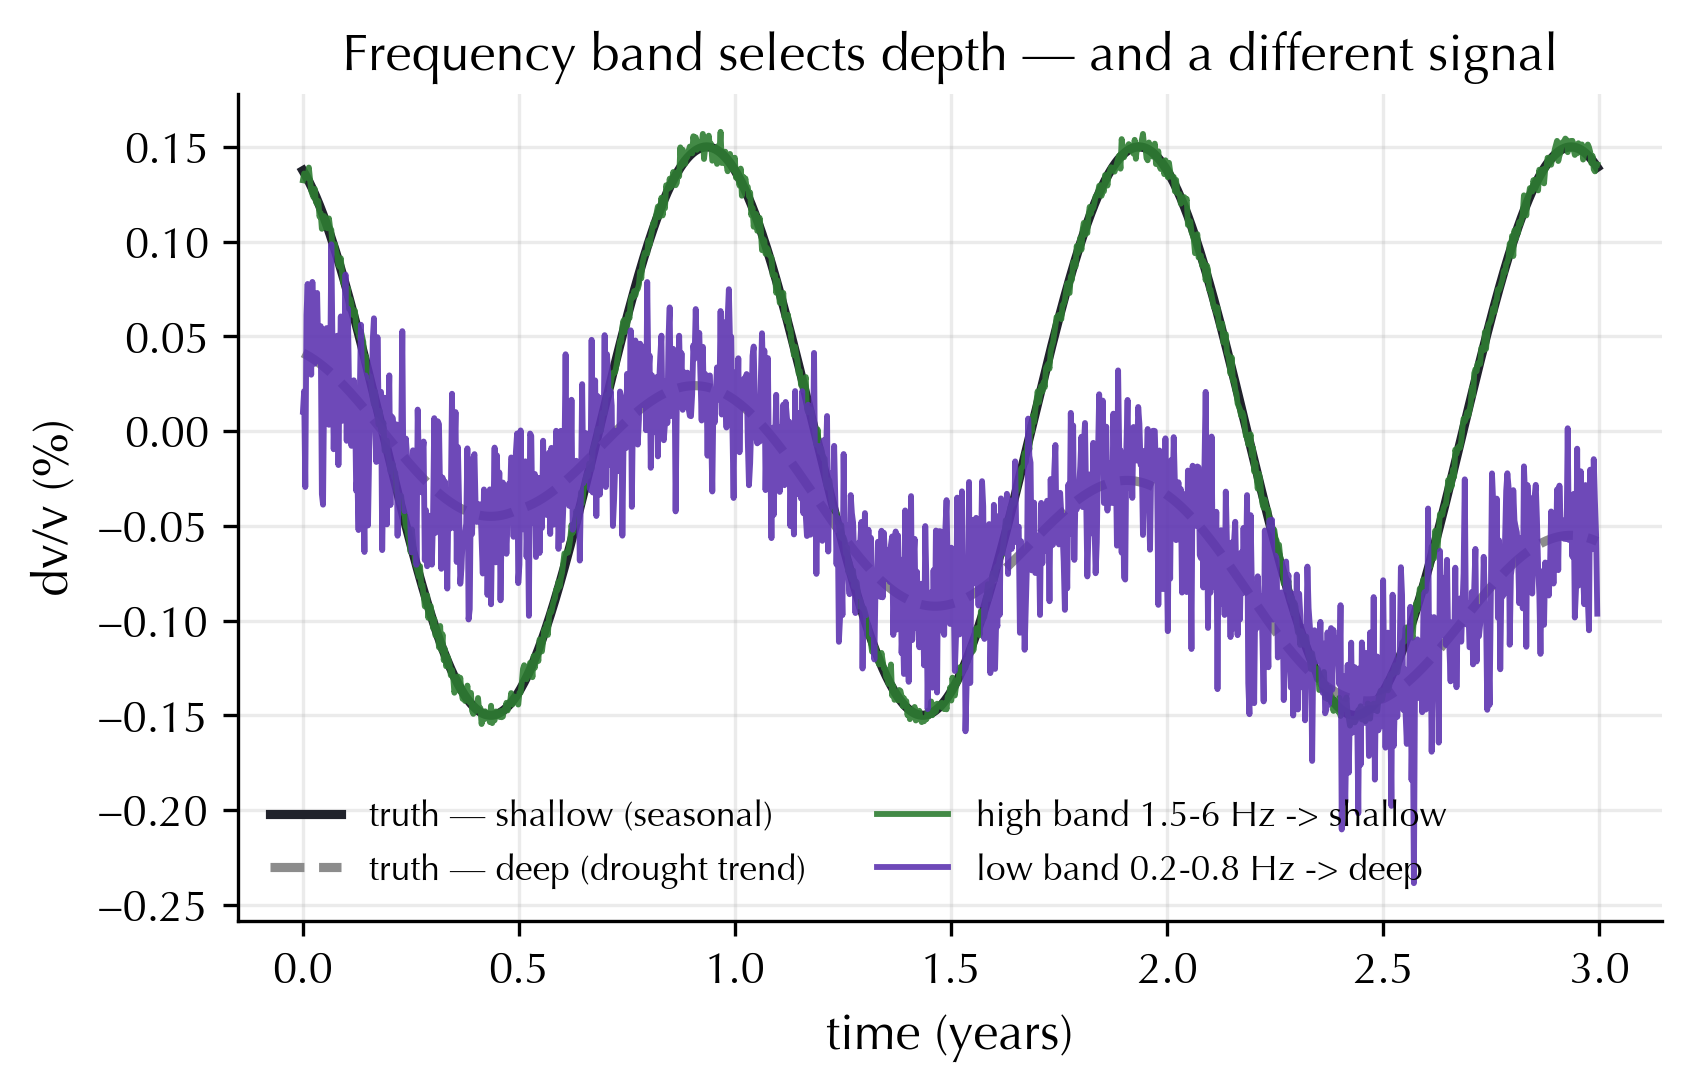
\includegraphics[width=0.49\textwidth]{demo_4_frequency_depth.png}\hfill
  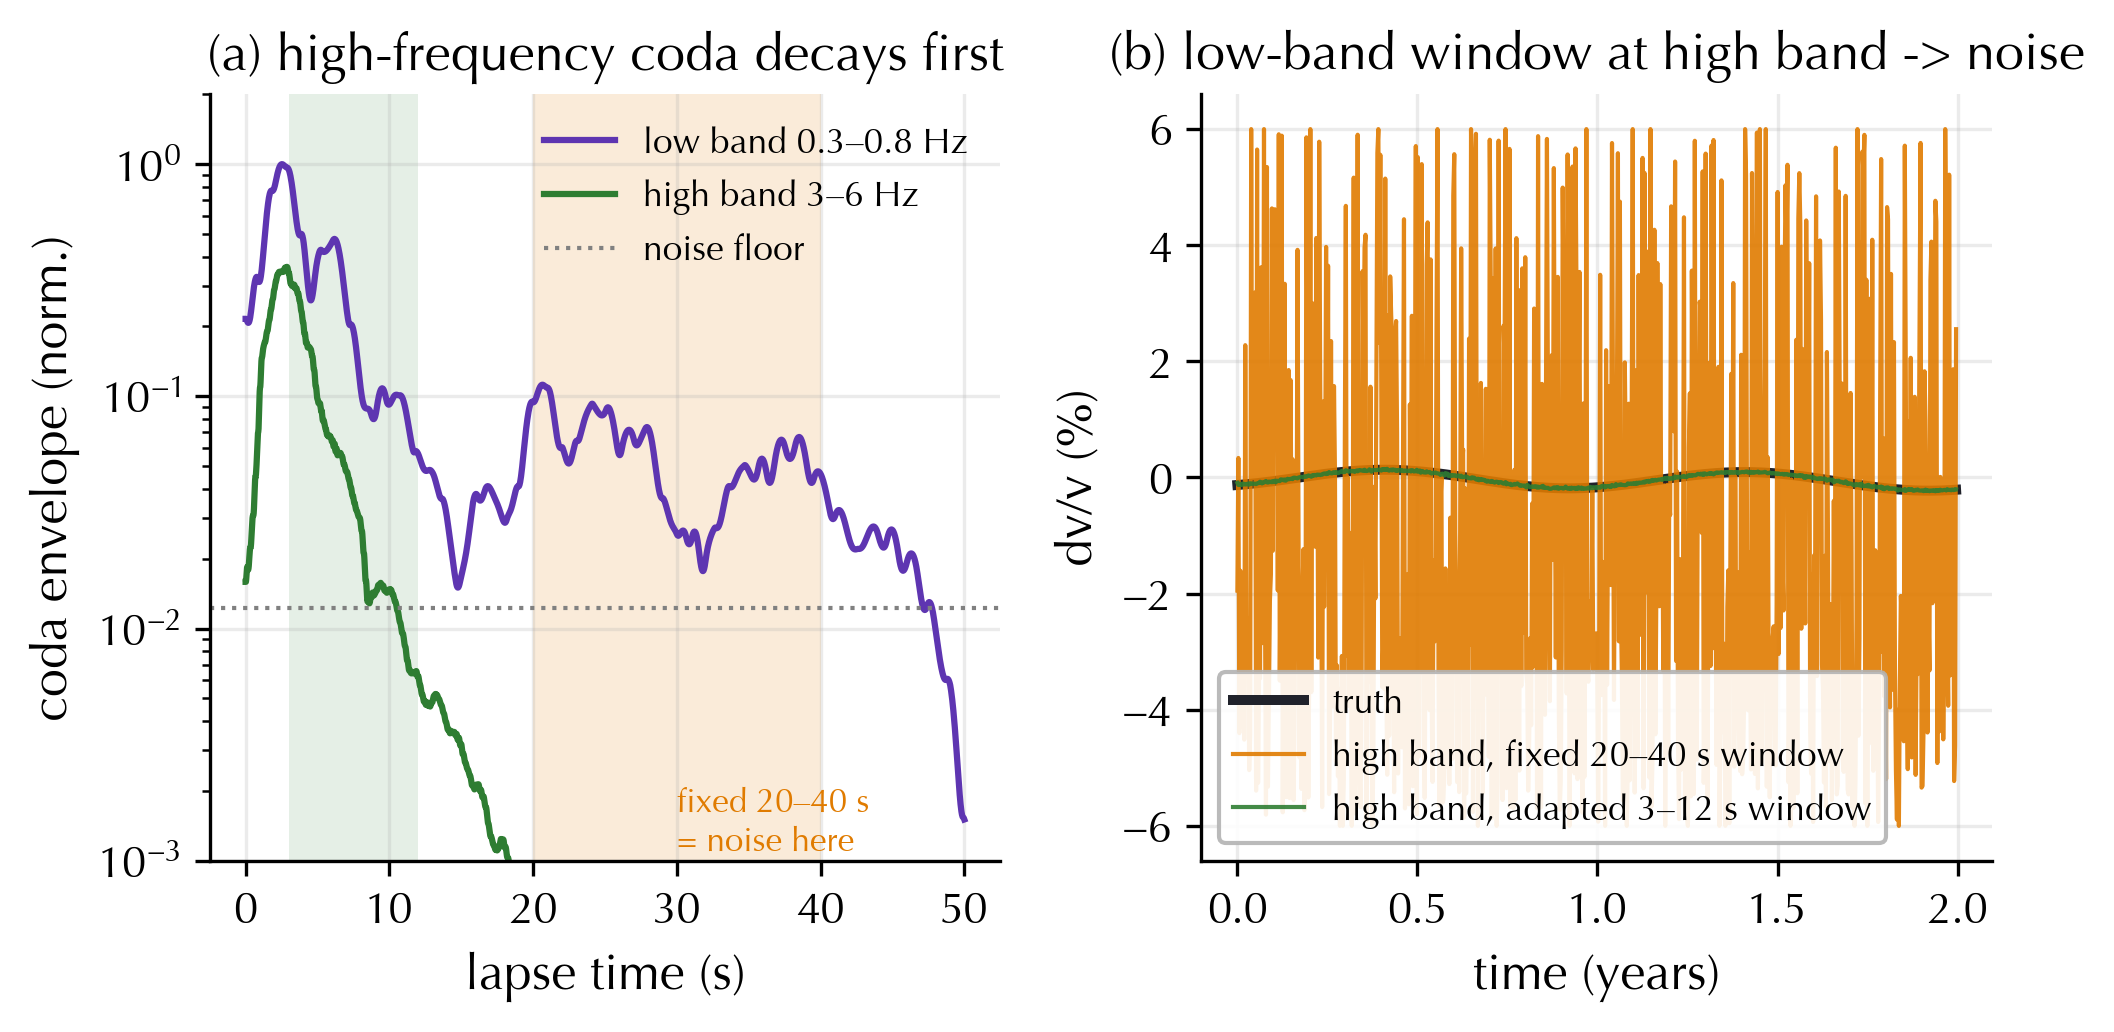
\includegraphics[width=0.49\textwidth]{demo_5_window_band.png}\\[2pt]
  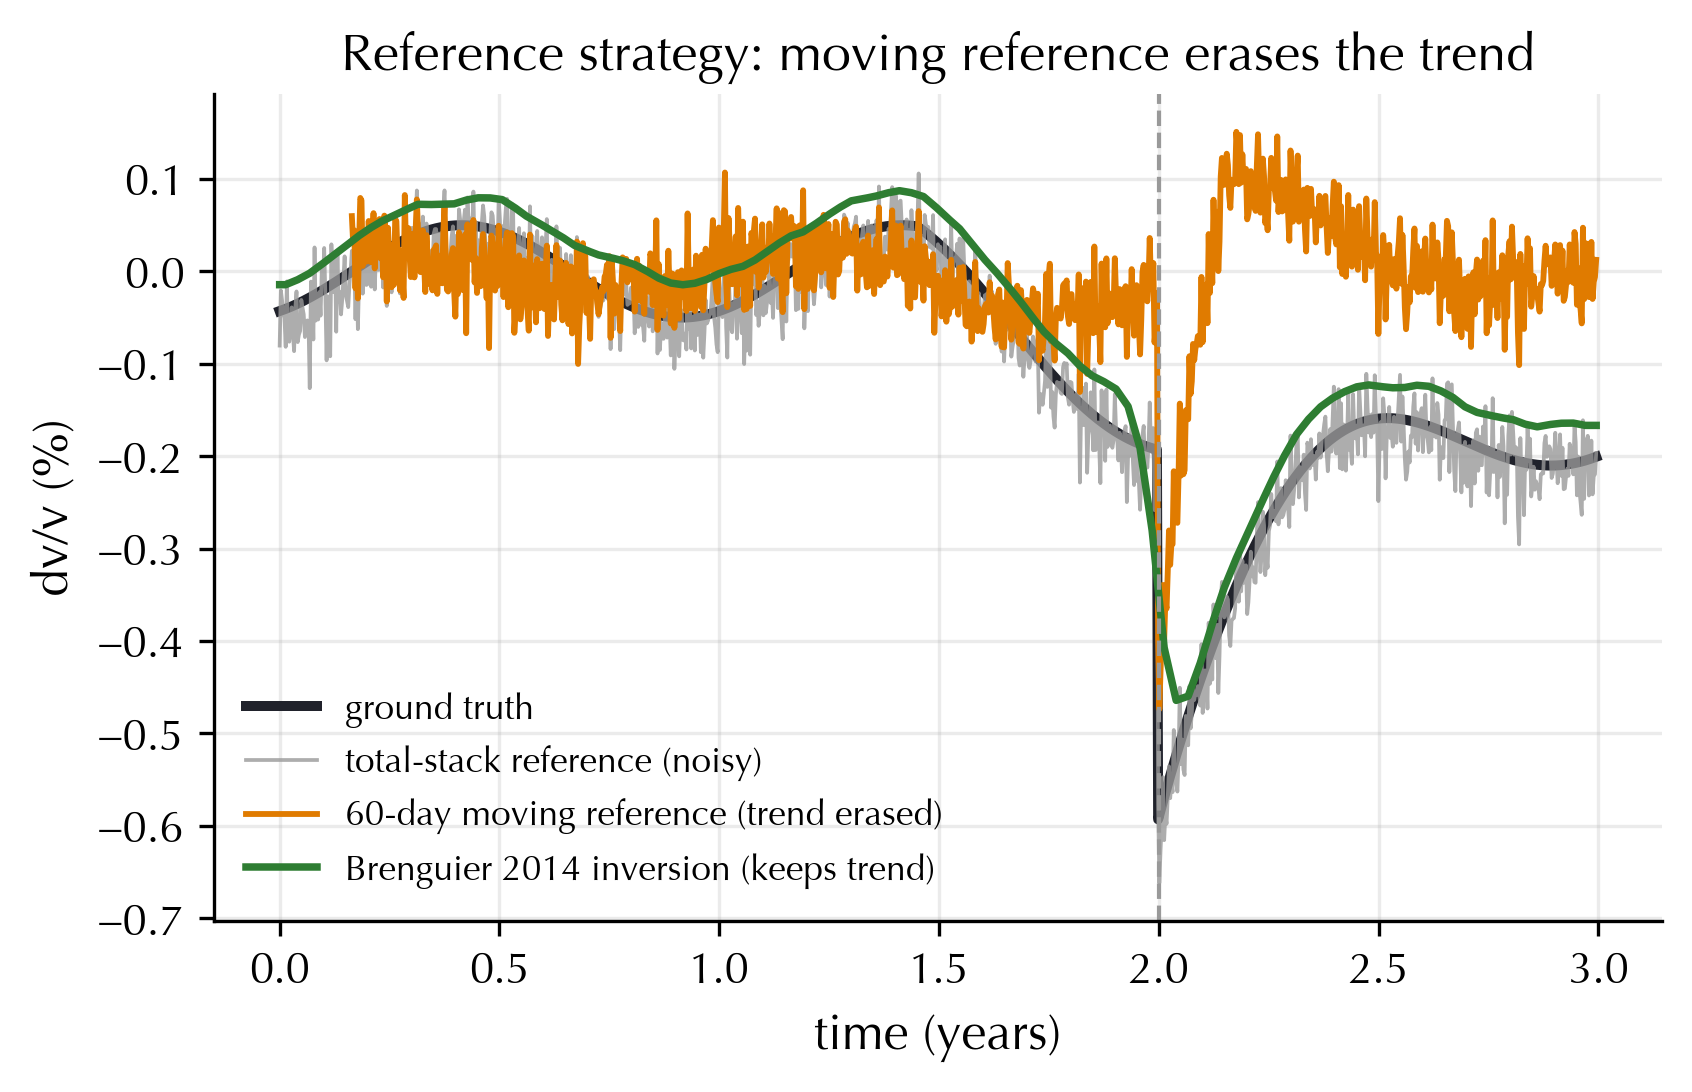
\includegraphics[width=0.49\textwidth]{demo_7_reference.png}\hfill
  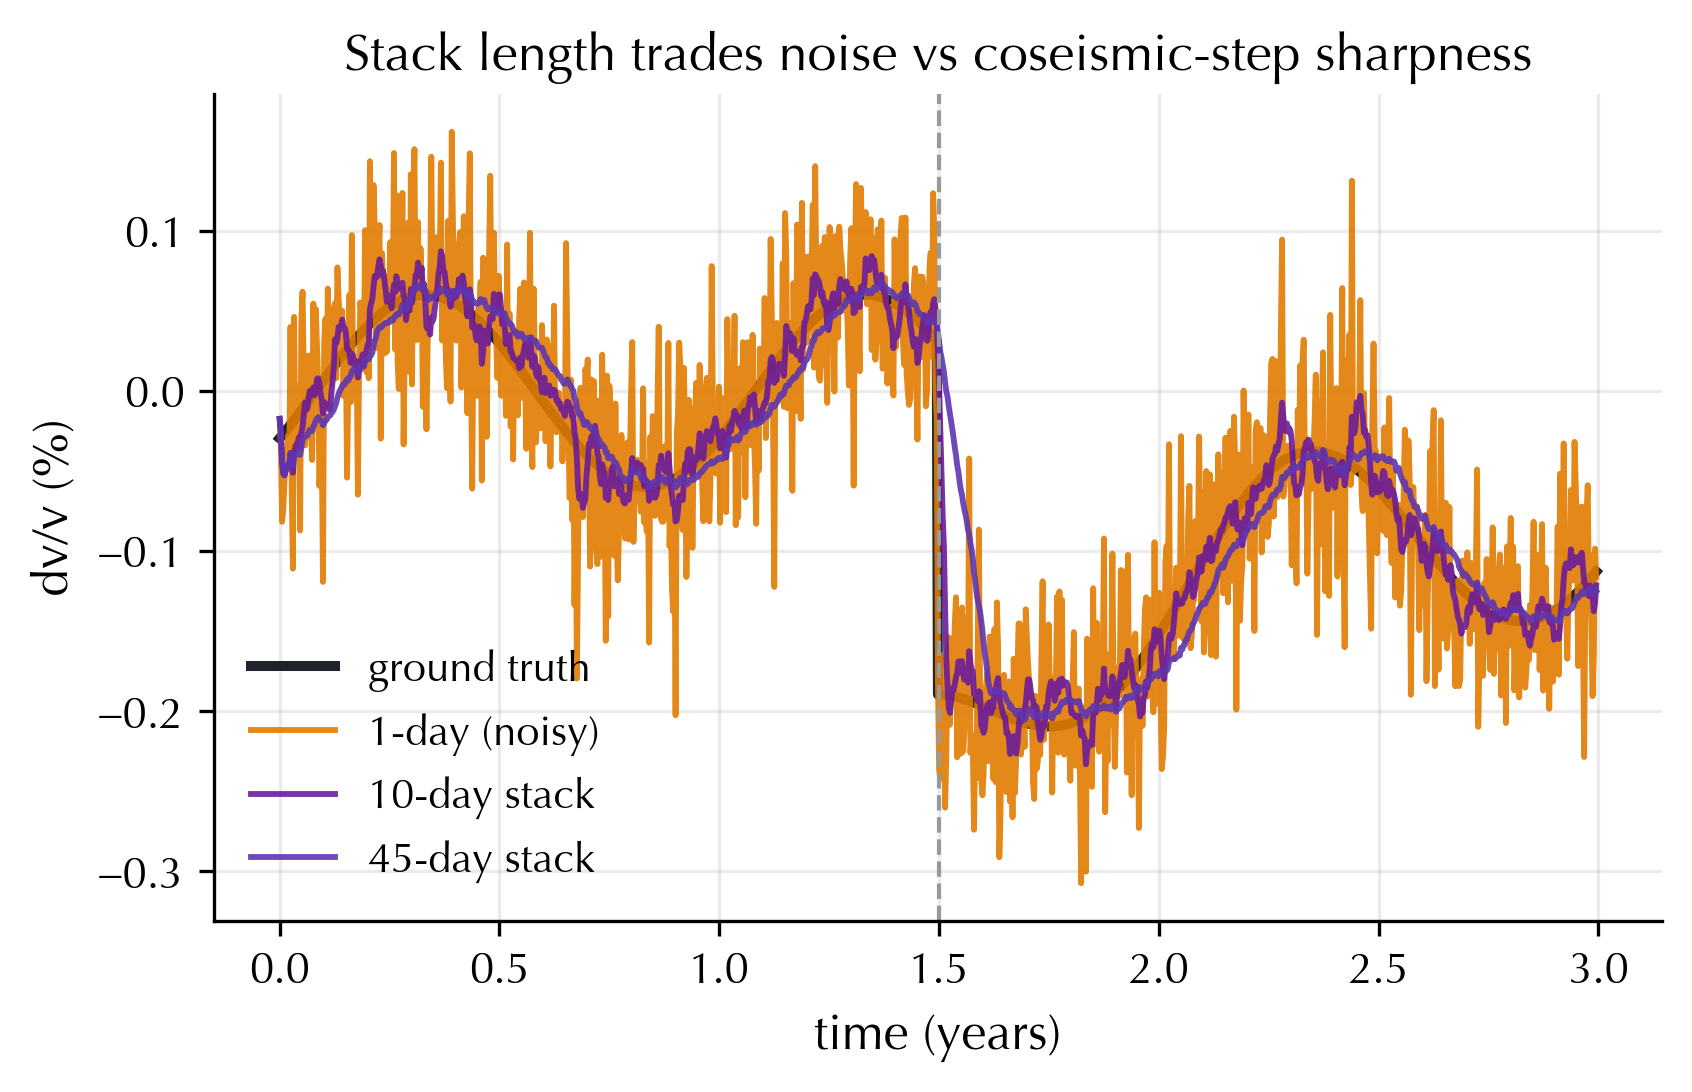
\includegraphics[width=0.49\textwidth]{demo_6_stacking.png}
  \caption{Parameter choices. (a) Frequency band selects depth and signal. (b)
  A coda window does not transfer across bands. (c) Reference strategy: a moving
  reference erases the trend a fixed reference and the joint inversion keep. (d)
  Stacking length smears the coseismic step.}
  \label{fig:params}
\end{figure}

\subsection{\texorpdfstring{Choices that create spurious
\texorpdfstring{\dvv}{dv/v}}{Choices that create spurious }}\label{sec:artifacts}

Some choices do not merely bias the result --- they create spurious
signal. A station clock error delays the whole correlation by a
lapse-independent shift, producing an apparent \dvv~that appears with
opposite sign on the causal and acausal branches; measuring the two
branches separately is the diagnostic
(Fig.\textasciitilde{}\ref{fig:artifacts}a). Seasonally varying noise
sources warp the low-SNR late coda, so a late measurement window reports
a coherent spurious \emph{seasonal} \dvv~many times the real signal
while an earlier window stays clean \citep[the waveform-level version
of][]{Zhan2013} (Fig.\textasciitilde{}\ref{fig:artifacts}b).

\begin{figure}
  \centering
  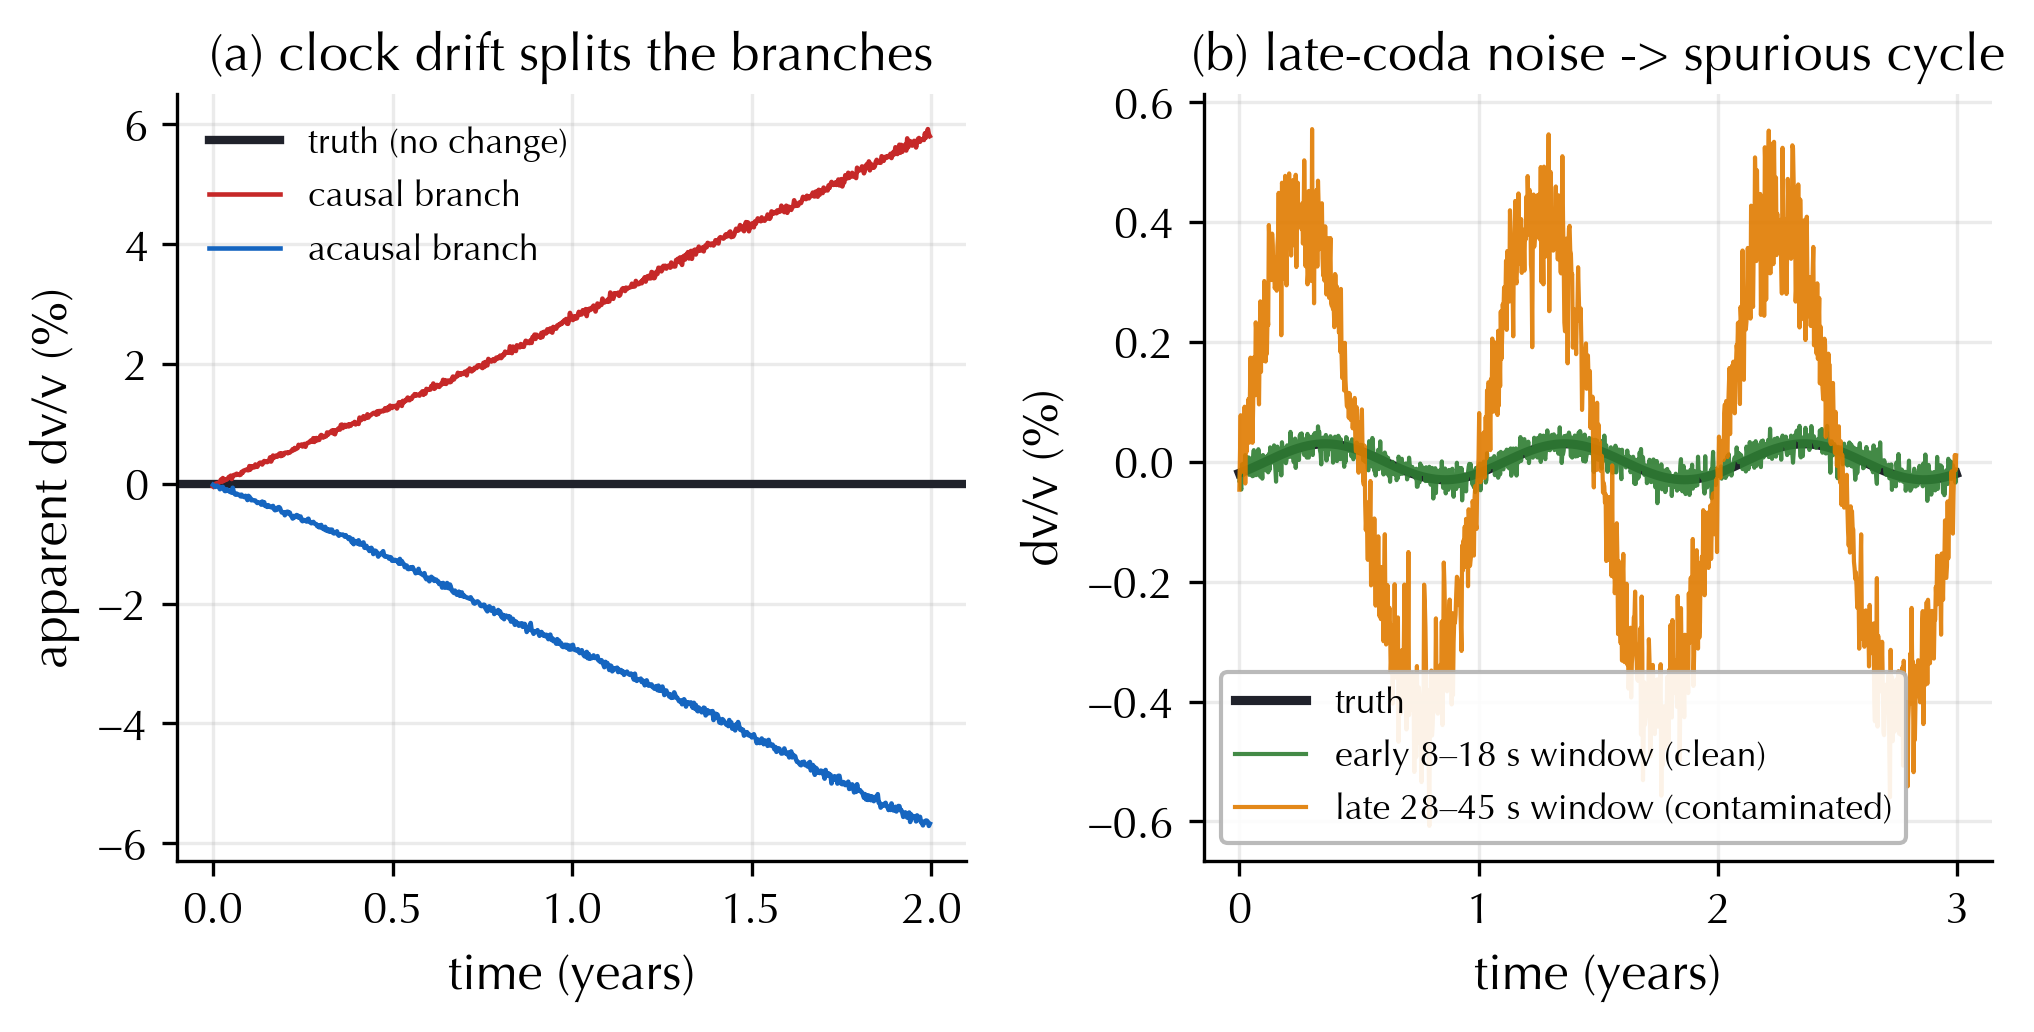
\includegraphics[width=\textwidth]{demo_8_artifacts.png}
  \caption{Deviations that create spurious \dvv. (a) A clock drift splits the causal
  and acausal branches with opposite sign. (b) Seasonal late-coda noise injects a
  spurious seasonal \dvv\ into a late window but not an early one.}
  \label{fig:artifacts}
\end{figure}

\subsection{Causal and acausal branches: a further aggregation
choice}\label{sec:branches}

The clock-error diagnostic above uses the two branches of the
correlation, and how they are \emph{combined} is itself an
under-reported choice. The causal (positive-lag) and acausal
(negative-lag) branches sample opposite-direction paths with different
source-side illumination, and in a 3D medium their sensitivity kernels
sample partly different volumes, so the two can report genuinely
different \dvv~without either being wrong. Two regimes bound the choice
(Fig.\textasciitilde{}\ref{fig:branches}). When a change is
\emph{localized} to the volume one branch samples, symmetrizing or
averaging the branches --- the common default --- dilutes it toward
zero, while the branch that carries the change recovers it
(Fig.\textasciitilde{}\ref{fig:branches}a); here preferring the branch
of greatest change is recovering a real quantity. When instead both
branches share the \emph{same} change, their difference is measurement
noise, and selecting the branch of greatest change over-reports it --- a
max-of-two-estimators selection bias that grows as SNR falls
(Fig.\textasciitilde{}\ref{fig:branches}b). The rule ``take the side of
the greatest change'' therefore helps only after a structural check: the
two branches must change with the \emph{same sign} (opposite signs are a
clock error, Fig.\textasciitilde{}\ref{fig:artifacts}a) and be coherent
in time. The defensible procedure is to measure both branches, gate on
that consistency, select by the coherence of the change rather than its
amplitude (a criterion independent of the answer, so it carries no
selection bias), and carry the between-branch difference as an explicit
term of the measurement covariance \(C_d\)
(Section\textasciitilde{}\ref{sec:bayes}) rather than discarding it by
averaging.

\begin{figure}
  \centering
  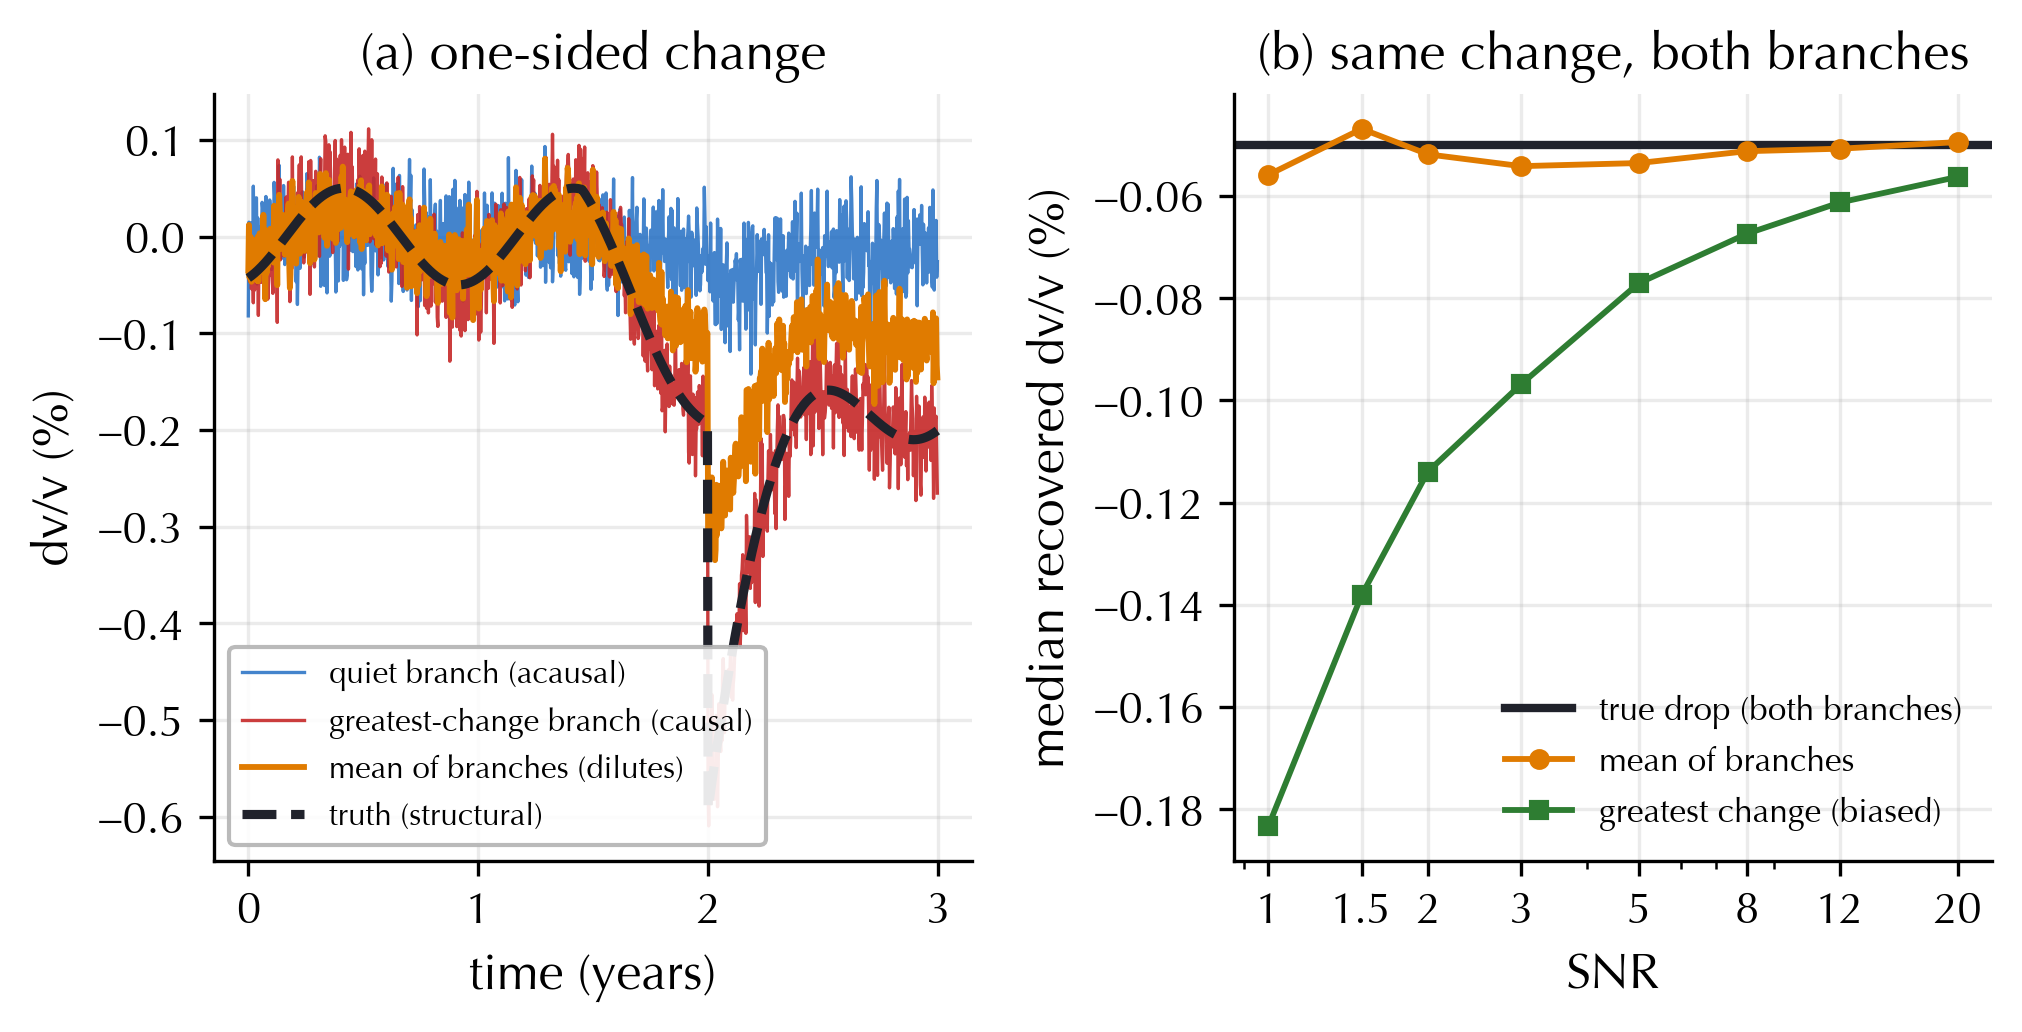
\includegraphics[width=\textwidth]{demo_13_branch_asymmetry.png}
  \caption{Combining the causal and acausal branches. (a) A change localized to
  the volume the causal branch samples: averaging the branches dilutes it to
  about half, while the branch carrying it recovers the truth. (b) The same
  change on both branches: selecting the branch of greatest change over-reports
  the drop, worsening as SNR falls (a selection bias), while the branch mean
  stays unbiased.}
  \label{fig:branches}
\end{figure}

Taken together, the choices compound. We make this concrete in
Section\textasciitilde{}\ref{sec:multiverse} by running the full
\emph{multiverse} of best-practice and deviation choices on one
synthetic dataset and ranking each by the bias and the error-bar change
it induces.

\section{The multiverse of processing choices}\label{sec:multiverse}

The figures so far each isolate one choice. We now ask the cumulative
question directly. Starting from a single \textbf{best-practice
baseline} (trace stretching, a band matched to the target depth, a coda
window well past the direct arrival, a 10-day stack, a long stable
reference, coherence gating; the cross-cutting rules of
\citeauthor{Brenguier2014}
\citetext{\citeyear{Brenguier2014}; \citealp{Weaver2011}; \citealp{Clarke2011}}
as distilled in our survey), we flip \emph{one} choice at a time to a
documented deviation and measure the resulting error against the known
truth (Fig.\textasciitilde{}\ref{fig:deviations}). The ranking is
unambiguous: relative to a best-practice RMS error of
\(\sim\!0.02\,\%\), an unwrapped phase estimator that cycle-skips is
catastrophic, a moving reference and a wrapped-phase MWCS each inflate
the error roughly an order of magnitude, an over-long stack and a late
low-SNR window distort the co-eruptive drop, while the frequency band
(which mostly sets precision here) and the gating are second-order. The
Brenguier joint inversion is nearly as good as the fixed reference and
preserves the trend.

\begin{figure}
  \centering
  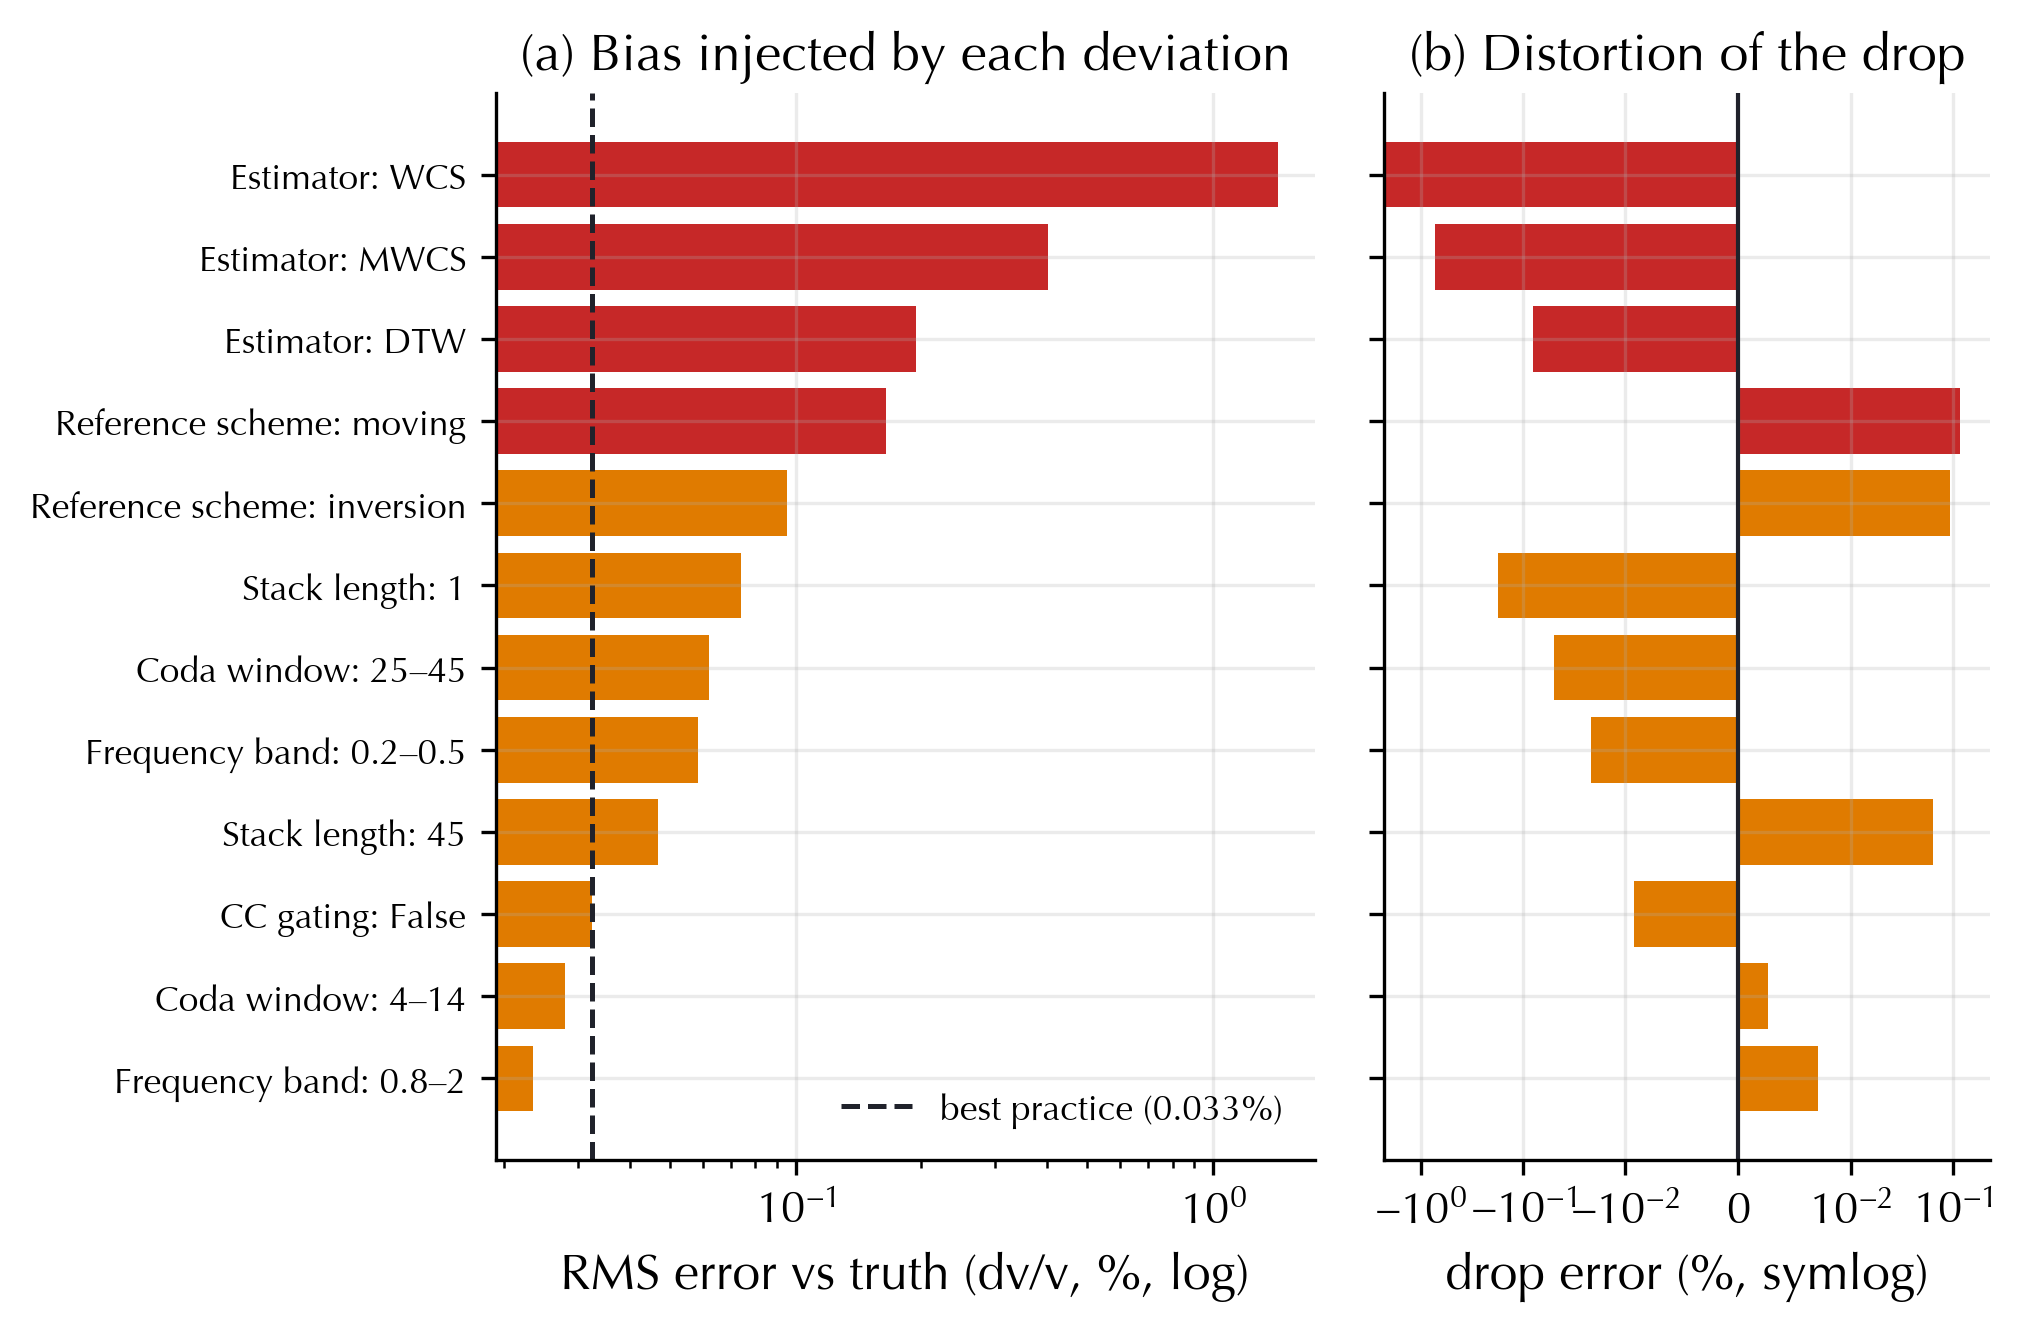
\includegraphics[width=\textwidth]{demo_10_deviations.png}
  \caption{One-at-a-time deviations from a best-practice baseline, ranked by the
  bias they inject (a, log scale) and by how they distort the recovered
  co-eruptive drop (b, symlog). Bars are coloured red when the error exceeds
  three times the baseline. The estimator and reference choices dominate; the
  band and gating are minor for this scenario.}
  \label{fig:deviations}
\end{figure}

The choices do not act in isolation, so we run the \textbf{full
factorial}: every combination of three estimators, two bands, three coda
windows, three stack lengths and two reference schemes --- 108
individually reasonable pipelines --- on one volcano dataset
(Fig.\textasciitilde{}\ref{fig:multiverse}a). The recovered \dvv~fans
out across more than an order of magnitude in RMS error, and the fan is
widest exactly at the sharp co-eruptive drop. Attributing the variance
of the outcome to each axis with a first-order (main-effect) sensitivity
index (Fig.\textasciitilde{}\ref{fig:multiverse}b) shows that, for this
dataset, the \textbf{coda window and the stack length} control the RMS
error most, the \textbf{stack length} dominates the recovered drop
amplitude, and the estimator is third; the first-order indices sum to
well under one, so a large part of the spread is \emph{interaction}
between choices --- compounding, not additive. The appropriate object is
therefore not a single curve but a distribution of \dvv~over the
processing choices.

\begin{figure}
  \centering
  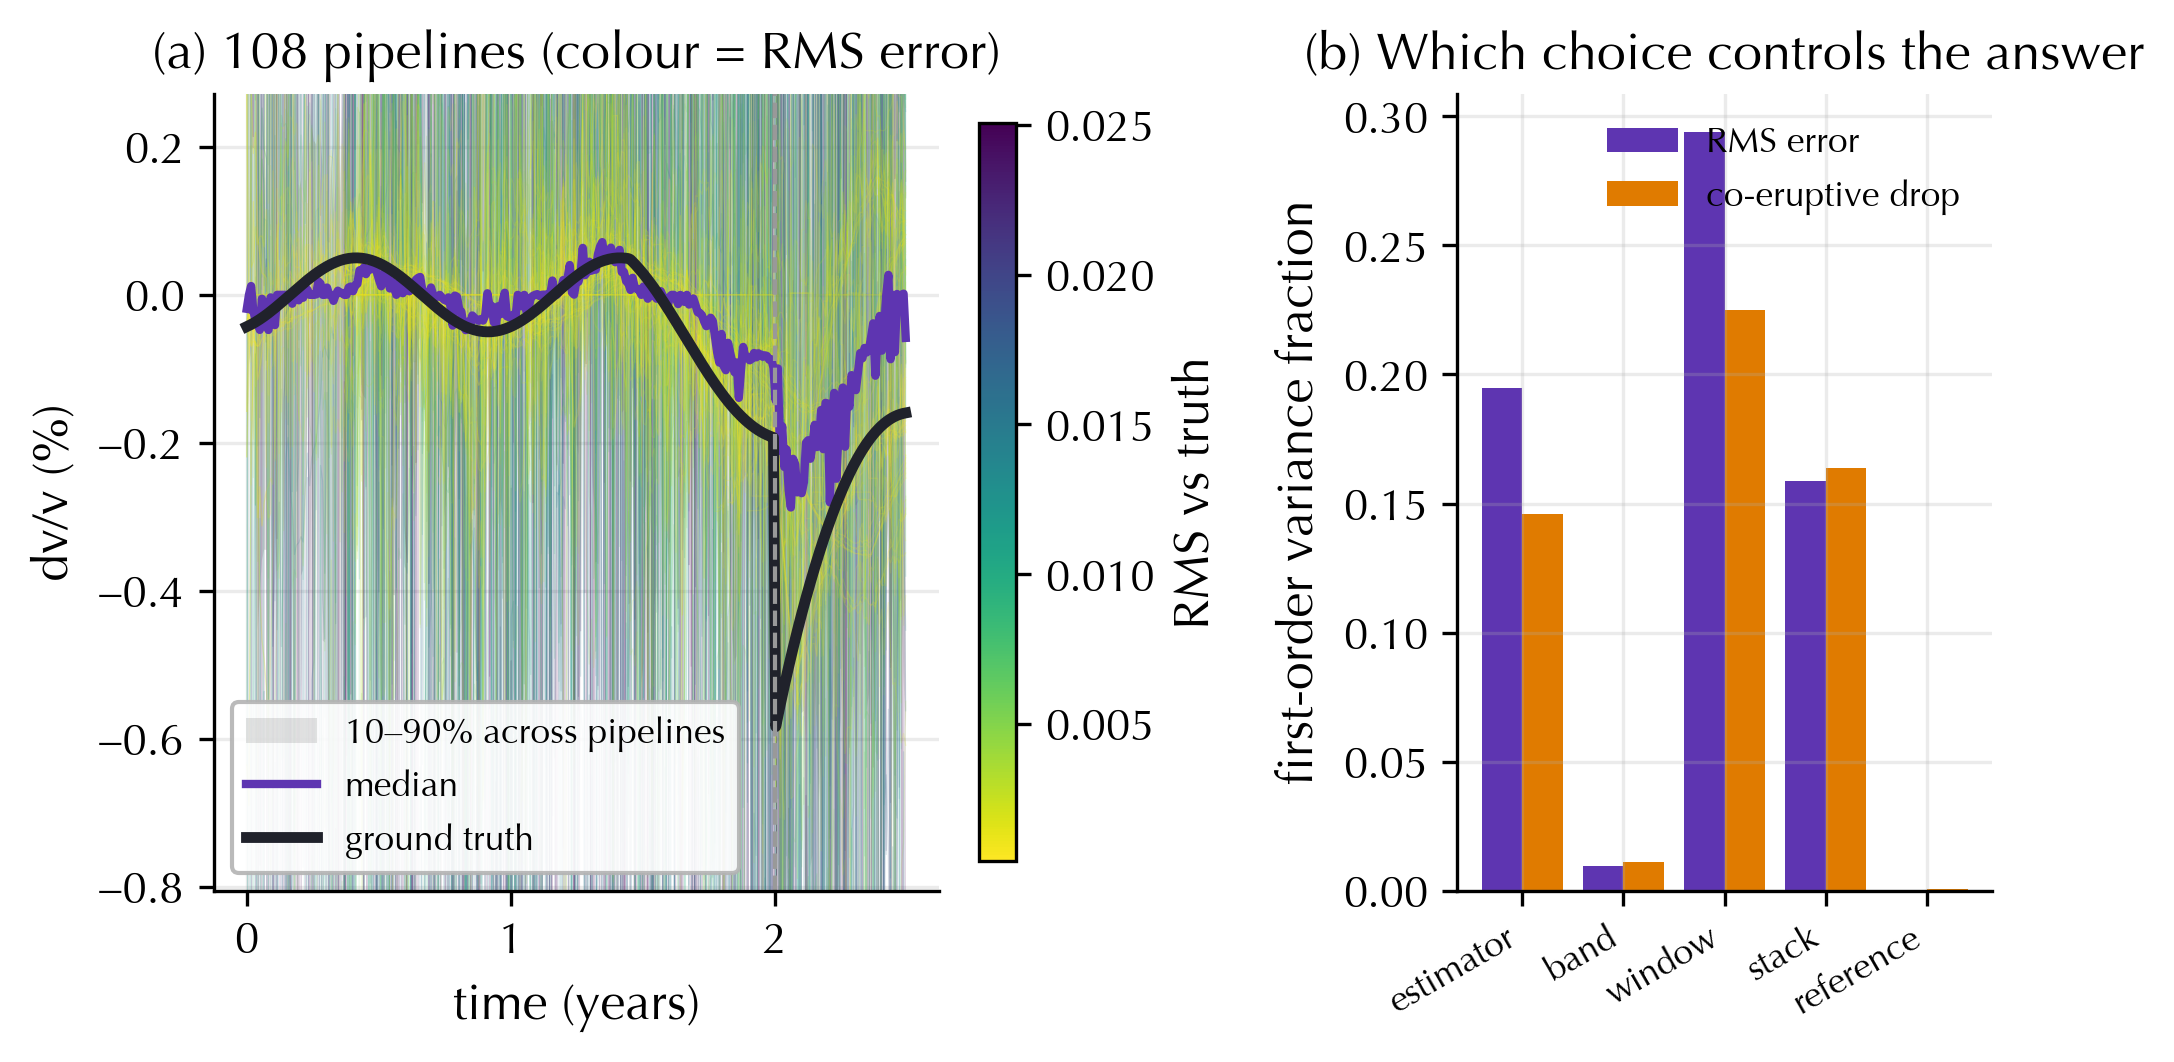
\includegraphics[width=\textwidth]{demo_11_multiverse.png}
  \caption{The full multiverse. (a) 108 reasonable pipelines on one dataset,
  each coloured by its RMS error against the truth on a colourblind-safe scale
  (bright accurate, dark biased; the worst run off the clipped axis); the grey band
  is the 10--90\% inter-pipeline spread, widest at the velocity drop. (b) First-order variance attribution: which
  choice controls the RMS error and the recovered drop. Window and stack length
  dominate; the sub-unity sum signals strong interactions.}
  \label{fig:multiverse}
\end{figure}

Table\textasciitilde{}\ref{tab:bp-measure} distils this into the
measurement-step best practice and the documented deviation for each
choice, with the consequence the synthetic makes concrete. The baseline
and deviation sets are the ones our survey extracts from the literature
(the cross-cutting rules of \citeauthor{Snieder2002}
\citetext{\citeyear{Snieder2002}; \citealp{Clarke2011}; \citealp{Weaver2011}; \citealp{Brenguier2014}; \citealp{Wang2017}; \citealp{Obermann2019}})
and that \texttt{codameter.deviations} runs.

\begin{table}
\footnotesize
\caption{Measurement step: best practice versus the common deviation and its
consequence. Rows are the axes swept in Fig.~\ref{fig:multiverse}; the sets
follow the literature survey (Appendix~\ref{app:survey}).}
\label{tab:bp-measure}
\begin{tabularx}{\textwidth}{@{}>{\raggedright\arraybackslash}p{2.5cm} L L L@{}}
\toprule
\textbf{Choice} & \textbf{Best practice} & \textbf{Common deviation} &
\textbf{Consequence} \\
\midrule
Estimator & Stretching family (TS/WTS/WCC), robust at low SNR and large \dvv\
\citep{Mikesell2015,Yuan2021} & Wrapped-phase MWCS \citep{Clarke2011} without 2-D
unwrapping \citep{Mao2020} & Cycle-skips at large \dvv; error inflated
$\sim\!10\times$ or catastrophic \\ \hline
Frequency band & Matched to the target depth: $\sim\!0.1$--2\,Hz (volcano, crust),
2--4\,Hz (aquifer), 4--12\,Hz (shallow damage) \citep{Obermann2013,Obermann2016} &
Off-target or a single wide band & Mixes depths; here mostly sets precision \\ \hline
Coda window & Lapse window past the direct arrival, scaled with the band:
$\sim\!5$--30\,s (crustal) up to $\sim\!100$\,s (station pairs) \citep{Obermann2013} &
Fixed late window reused across bands & Measures noise at high $f$; bias and
inflated $\sigma$ \\ \hline
Stack length & Short enough to resolve the transient ($\sim\!10$\,d), on a long,
stable reference span \citep{Wang2017} & Over-long stack ($\sim\!45$\,d) & Smears and
delays a step; distorts the recovered drop \\ \hline
Reference & Long fixed stack or all-to-all joint inversion
\citep{Brenguier2014,Wang2017} & Moving / trailing reference & Erases slow trends \\ \hline
Coherence gating & Discard low-coherence epochs (CC / SNR threshold)
\citep{Clarke2011} & No gating & Keeps corrupted epochs; changes the effective $N$ \\ \hline
Uncertainty definition & State it explicitly: within-measurement
\citep{Weaver2011,Clarke2011} / SE / SD & Left unstated & Factor $\sqrt{N}$
ambiguity in significance (Fig.~\ref{fig:uncertainty}) \\
\bottomrule
\end{tabularx}
\end{table}

\section{A Bayesian measurement model and its data
covariance}\label{sec:bayes}

If the processing choice controls the answer, the principled response is
not to select a single pipeline but to treat the choice as a
\textbf{nuisance parameter} with a prior and marginalise it out. We
propose this as the new best practice for the \dvv~\emph{measurement},
and implement it as a Bayesian hierarchical inversion. For configuration
\(k\) drawn from a prior over reasonable pipelines we obtain a measured
series \(m_k(t)\) with a coherence-limited within-method floor
\(\sigma_k(t)\) \citep{Weaver2011, Clarke2011}, and posit
\begin{equation}
m_k(t) = \mu(t) + \beta_k + \varepsilon_k(t), \qquad
\beta_k\sim\mathcal N(0,\tau^2),\quad
\varepsilon_k(t)\sim\mathcal N\!\big(0,\,s^2\sigma_k(t)^2\big),
\label{eq:bayes}
\end{equation} with a second-difference random-walk smoothness prior on
the latent true series \(\mu(t)\). Here \(\beta_k\) is configuration
\(k\)'s methodological bias (the systematic offset between, say, MWCS
and stretching), \(\tau\) its scale across the ensemble, and \(s\)
rescales the Weaver floor so the data report whether it is calibrated. A
conjugate Gibbs sampler returns the joint posterior; the implementation
is \texttt{codameter.uq\_bayes} (pure NumPy, no external sampler).

The model yields two distinct objects, and conflating them is the error
the field makes (Fig.\textasciitilde{}\ref{fig:bayes}). The posterior of
\(\mu\) is the precision of the \emph{combined} estimate: it is tight
and shrinks with ensemble size --- yet it \emph{under-covers the truth},
because the configurations share a common-mode bias that averaging
cannot remove. The object a downstream depth or stress inversion must
consume is the \textbf{marginal measurement covariance} \begin{equation}
C_d(t,t') = \underbrace{D R D}_{\text{within}\,\oplus\,\text{methodological},\ \text{temporally correlated}}
\;+\; \underbrace{\tau^2\,\mathbf{1}\mathbf{1}^\top}_{\text{common mode}},
\qquad D=\operatorname{diag}\!\big(\sigma_{\rm tot}(t)\big),
\label{eq:cd}
\end{equation} with \(\sigma_{\rm tot}^2 = s^2\sigma_k^2\)-average \(+\)
methodological variance and \(R_{ij}=e^{-|t_i-t_j|/L}\) for a
correlation length \(L\) estimated from the ensemble residuals. This
\(C_d\) is \textbf{time-dependent} --- wider at the sharp drop and at
low coherence --- and its temporal correlation plus common-mode term
collapse the effective number of independent epochs by an order of
magnitude. On our synthetic the marginal \(C_d\) covers the truth at the
nominal rate while the naive posterior band does not, making concrete
that the \emph{measurement covariance}, not the posterior of the
averaged series, is what must be propagated.

\begin{figure}
  \centering
  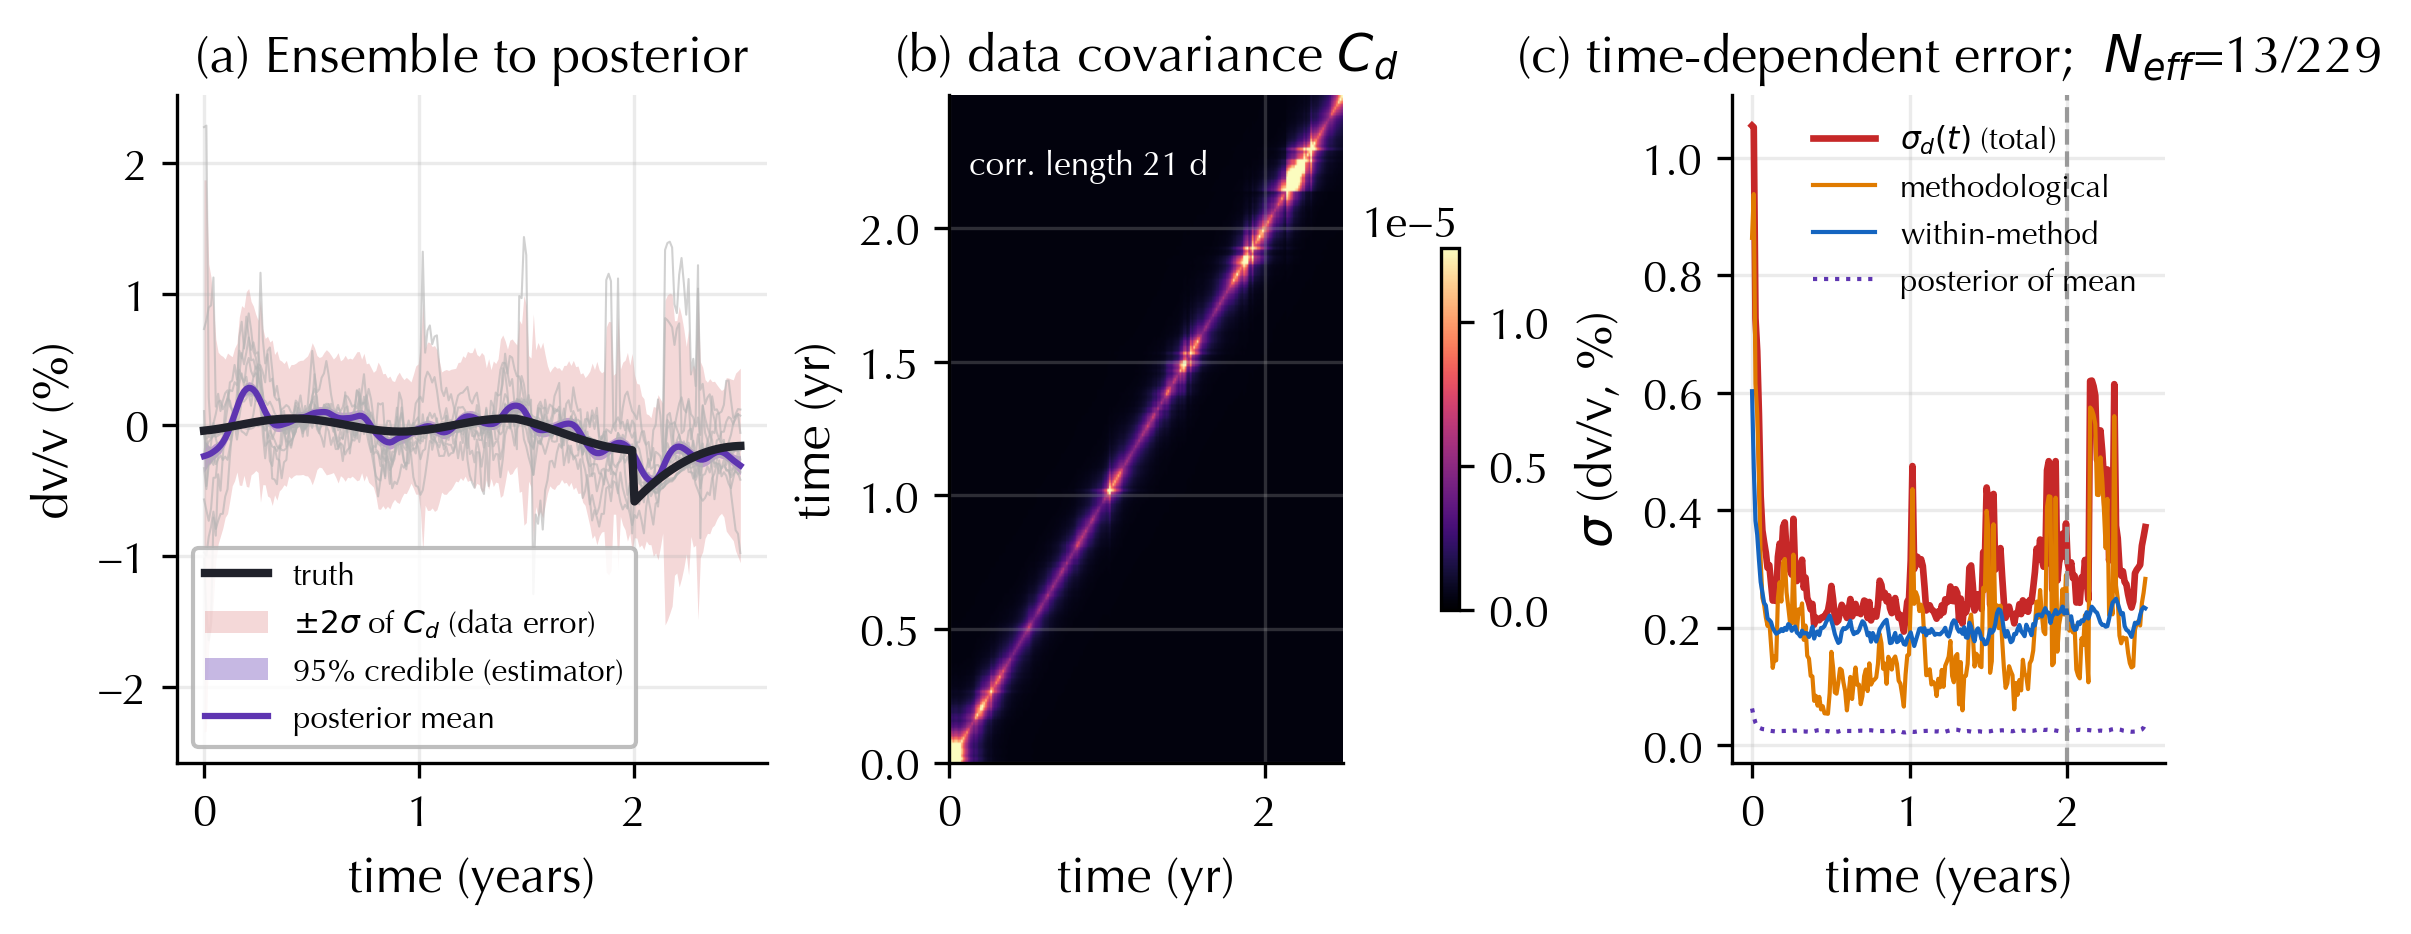
\includegraphics[width=\textwidth]{demo_12_bayes.png}
  \caption{The Bayesian measurement model. (a) The processing ensemble (grey)
  is marginalised into a posterior mean (purple) with a narrow credible band
  (the estimator precision) and a much wider $\pm2\sigma$ band from the marginal
  $C_d$ (the honest data error), which covers the truth where the credible band
  does not. (b) The resulting time-dependent data covariance $C_d$. (c) Its
  diagonal $\sigma_d(t)$ decomposed into within-method and methodological parts,
  rising at the eruption; the posterior-of-the-mean (dotted) is far tighter, and
  $N_{\rm eff}$ is a fraction of the epoch count.}
  \label{fig:bayes}
\end{figure}

\section{Depth: propagating the measurement covariance through
sensitivity kernels}\label{sec:depth}

The remaining sections present a framework rather than new synthetics:
they set out how the covariance of
Section\textasciitilde{}\ref{sec:bayes} propagates down the inference
chain, and ground each step in what the monitoring literature does and
does not yet report. The executable stages are in development in the
open codameter package (Section\textasciitilde{}\ref{sec:discussion}).

The field has converged on one physical rule for depth --- \emph{depth
is set by the frequency band and the coda lapse time, it is not assumed}
\citep{Obermann2013, Obermann2016} --- and, increasingly, on multi-band
measurement as the means to resolve it
\citep{Takano2017, Feng2020, Mao2022}. The step from a set of per-band
\dvv~series to a depth profile is where reporting is least consistent:
many studies read a single band as a single depth, only a few invert
several bands against surface-wave sensitivity kernels, and the
propagation of the measurement error into the depth estimate is seldom
shown. The depth assignment is frequently the scientific claim itself
--- whether the change lies in the aquifer or the overlying soil,
whether coseismic softening is a shallow site response or slip on the
fault at depth \citep{Rubinstein2005} --- so a depth reported without
its uncertainty cannot support that claim.

A \dvv~measured in band \(b\) is not a point sample but a weighted
integral over depth, \begin{equation}
\Big(\tfrac{\delta v}{v}\Big)_b = \int_0^\infty K_b(z)\,\frac{\delta V_S}{V_S}(z)\,\mathrm{d}z \;+\; \varepsilon_b,
\label{eq:kernel}
\end{equation} where \(K_b(z)\) is the (Rayleigh-wave) depth-sensitivity
kernel for band \(b\) and \(\varepsilon_b\) carries that band's
measurement covariance from Section\textasciitilde{}\ref{sec:bayes}.
Stacking bands gives a linear system
\(\mathbf{d}=\mathbf{G}\,\mathbf{m}+\boldsymbol\varepsilon\) with
\(\mathbf{G}_{bz}=K_b(z)\) and data covariance \(C_d\); the Bayesian
solution under a smoothness prior returns a depth profile
\(\delta V_S/V_S(z)\) together with its posterior covariance \(C_m(z)\)
(implemented in \texttt{codameter.uq\_depth}). The bands must sit where
the kernels resolve: too low and the kernel leaks into the half-space,
too high and the coda is incoherent
(Section\textasciitilde{}\ref{sec:params}). The width of \(C_m(z)\) ---
not the profile alone --- is the deliverable, and it inherits the
temporal correlation and common-mode structure of \(C_d\).

One assumption is usually left implicit: that a \dvv~change is a
shear-velocity change alone. In partially saturated ground it is not.
Filling or draining pore space changes both the shear modulus and the
bulk density, so for the shear-dominated coda the observed change mixes
the two, \begin{equation}
\frac{\delta v}{v} \;\approx\; \tfrac12\frac{\delta\mu}{\mu} \;-\; \tfrac12\frac{\delta\rho}{\rho},
\label{eq:density}
\end{equation} and velocity alone cannot separate them. A petrophysical
model --- Gassmann fluid substitution for the modulus and a
porosity--saturation relation for the density
\citep{Gassmann1951, Mavko2009} --- is what breaks the degeneracy, at
the cost of its own prior uncertainty on porosity, fluid modulus, and
the saturation path. Hydrological and cryospheric targets, where
saturation varies strongly \citep{Clements2018, James2019}, are
precisely where neglecting the density term biases the inferred velocity
change and, downstream, the stress. The framework carries
\(\delta\rho/\rho\) as a second inverted field with its own kernel and
reports how much of the surface \dvv~each explains; the executable
version is a documented extension
(Section\textasciitilde{}\ref{sec:discussion}).

\begin{table}
\footnotesize
\caption{Depth step: best practice versus the common deviation in going from
per-band \dvv\ to a depth profile, and the consequence for the interpretation.}
\label{tab:bp-depth}
\begin{tabularx}{\textwidth}{@{}>{\raggedright\arraybackslash}p{2.6cm} L L L@{}}
\toprule
\textbf{Choice} & \textbf{Best practice} & \textbf{Common deviation} &
\textbf{Consequence} \\
\midrule
Depth assignment & Invert several bands against sensitivity kernels &
Read one band as one depth & No depth resolution and no depth error \\ \hline
Band selection & Bands where the kernels resolve (no half-space leak, coherent
coda) & Convenience band & Kernel leaks; unstable inversion \\ \hline
Measurement error & Propagate the per-band $C_d$ into the profile & Plot a profile
with no covariance & Overconfident depth attribution \\ \hline
Saturation & Separate $\delta V_S/V_S$ and $\delta\rho/\rho$ with a petrophysical
model in partly saturated ground & Assume a pure $\delta V_S/V_S$ change & Biased
velocity change and stress in hydrological and cryospheric targets \\ \hline
Velocity model & State the reference $V_P,V_S(z)$ and its uncertainty & Fixed,
unstated model & Hidden systematic in the kernels and the moduli \\
\bottomrule
\end{tabularx}
\end{table}

\section{Stress: from velocity change to stress and strain at
depth}\label{sec:stress}

The quantity of interest is rarely the velocity change itself but the
stress, strain, or pore-pressure change that produces it and ---
increasingly --- the forcing responsible for it. Here the literature
remains fragmented. Volcano and fault studies often interpret the
velocity change qualitatively (a pre-eruptive pressurization, coseismic
damage); hydrological studies fit an explicit poroelastic or
thermoelastic model and separate the two by their seasonal phase lag
\citep{Tsai2011, Wang2017, Clements2018}; and a growing body quantifies
stress sensitivity through an acoustoelastic coefficient
\citep{Brenguier2008, Nakata2011}. What is largely absent is the
\emph{uncertainty} on that final quantity and a reasonable apportionment
of it among the competing forcings. Because the material properties
entering the conversion are poorly constrained, the stress uncertainty
is dominated by \emph{epistemic} prior uncertainty rather than by the
measurement, so a stress value reported without it is the least
constrained quantity in the chain, and the one most often reported as a
result.

Velocity change is the acoustoelastic response to a stress change. Under
isotropic load the response is scalar ---
\(\delta v/v = \beta\,\varepsilon_{kk}\) with the bridge relation
\(\beta=-\mu'\kappa/2\mu\) (Denolle, in prep.) --- but in general it is
anisotropic, and the dominant fracture fabric selects \emph{which}
stress or strain component the velocity change tracks: a confining load
reads as volumetric strain, a directional stress reads as one deviatoric
component. Writing \(\beta_{ij}(z)\) for the acoustoelastic coefficient
of the fabric-selected component, the depth-resolved meter is
\begin{equation}
\Delta\sigma_{ij}(z,t) = \beta_{ij}(z)\,\frac{\delta V_S}{V_S}(z,t),
\label{eq:acoustoelastic}
\end{equation} with \(\beta_{ij}\) built from the layered moduli
\(\mu(z)=\rho V_S^2\), \(\kappa(z)=\rho\,(V_P^2-\tfrac43 V_S^2)\) and
the nonlinear sensitivity \(\mu'(z)\); the forward physics, its
drained/undrained regimes, and the fabric diagnostic that fixes
\(\beta_{ij}\) are the subject of the companion framework (Denolle, in
prep.). These coefficients are layered and weakly constrained ---
sometimes inferred from a tomographic \(V_P,V_S\) model --- so they
enter as \emph{per-layer priors}, and the stress covariance is the
Monte-Carlo pushforward of the depth posterior \(C_m(z)\) \emph{through}
those priors. This is the step where the aleatoric measurement chain and
the epistemic material priors merge; taking either alone understates the
stress uncertainty. Effective stress
(\(\Delta\sigma'=\kappa\,\varepsilon_{\rm vol}\) under isotropic load,
poroelastically clean) is the primary quantity; total stress adds a
poroelastic term \(\alpha_B\,\Delta p\) and is an optional extension.

Attribution --- how much of \(\Delta\sigma(z,t)\) is thermoelastic,
poroelastic, load, damage, or tectonic --- is deliberately \emph{not}
codameter's step. Each mechanism is a stress term that can act in
isolation, and decomposing the total into those terms is the
contribution of the companion unified-framework paper (Denolle, in
prep.), which supplies the forward models and the fabric diagnostic that
define \(\beta_{ij}\). codameter's role ends at delivering
\(\Delta\sigma_{ij}(z,t)\) with its posterior --- the input any such
decomposition must consume. The division of labour is well defined: this
paper is accountable for the measurement covariance and its propagation
to stress; the framework is accountable for the physics that turns that
stress into a named mechanism.

\begin{table}
\footnotesize
\caption{Stress step: best practice versus the common deviation in converting a
depth profile of velocity change to stress, with the consequence for the reported
result. Attribution of the stress to a forcing mechanism is the companion
framework's step and is not tabulated here.}
\label{tab:bp-stress}
\begin{tabularx}{\textwidth}{@{}>{\raggedright\arraybackslash}p{2.6cm} L L L@{}}
\toprule
\textbf{Choice} & \textbf{Best practice} & \textbf{Common deviation} &
\textbf{Consequence} \\
\midrule
Stress conversion & Acoustoelastic meter $\Delta\sigma_{ij}=\beta_{ij}(z)\,\delta V_S/V_S$
with layered $\beta_{ij},\mu'(z)$ priors & Single scalar coefficient, no prior &
Understated (epistemic) stress error \\ \hline
Stress component & Identify the fabric-selected component (isotropic vs deviatoric)
before inverting & Assume the isotropic $\delta v/v=\beta\varepsilon_{kk}$
everywhere & Wrong sign and magnitude under deviatoric load \\ \hline
Uncertainty budget & Merge the aleatoric depth covariance with the epistemic
material priors & Report the measurement error only & Stress error too small by
its dominant term \\ \hline
Stress measure & Report effective stress (poroelastically clean); flag any
total-stress assumptions & Conflate effective and total stress &
Non-comparable, ambiguous stress \\
\bottomrule
\end{tabularx}
\end{table}

\section{Discussion}\label{sec:discussion}

The experiments above share one finding: for ambient-noise \dvv, the
dominant control on both the reported value and its uncertainty is
frequently the \emph{processing choice}, not the data. This is a
consequential but tractable problem. We suggest three responses.

\textbf{Report the choices.} At minimum, a \dvv~study should state the
estimator and its parameters, the frequency band(s) and coda window(s)
and how the window was set relative to the band, the reference scheme,
the stacking, the cross-component and station-pair aggregation \emph{and
weighting}, and --- critically --- the exact definition of the quoted
uncertainty (within-measurement error, between-component/pair standard
error, or standard deviation). Our results show that the last item alone
can change a stated \(1\sigma\) by \(\sqrt{N}\).
Table\textasciitilde{}\ref{tab:checklist} collects this into a minimal
reporting checklist, and Appendix\textasciitilde{}\ref{app:survey} shows
how unevenly these items are reported across the literature today.

\begin{table}
\footnotesize
\caption{A minimal reporting checklist for an ambient-noise \dvv\ study. Stating
these turns an undocumented, irreproducible choice into an inspectable one and
makes error bars comparable across studies.}
\label{tab:checklist}
\begin{tabularx}{\textwidth}{@{}>{\raggedright\arraybackslash}p{3.4cm} L@{}}
\toprule
\textbf{Step} & \textbf{What to report} \\
\midrule
Pre-processing & Time-domain normalization (one-bit / running-mean), spectral
whitening band, sampling rate \\ \hline
Correlation \& stacking & Components computed, segment length, daily/sub-stack
length, total reference span \\ \hline
Estimator & Method (TS / WCC / DTW / MWCS / WCS / WTS / WTDTW), its parameters
($\varepsilon$-grid, or sub-window length and step), and whether the phase is
unwrapped \\ \hline
Frequency band(s) & $[f_1,f_2]$ for every reported measurement \\ \hline
Coda window(s) & $[t_1,t_2]$, the branch(es) used, and \emph{how} $t_1,t_2$ were
set relative to the band \\ \hline
Reference & Scheme (total stack / trailing / inversion) and period \\ \hline
Component aggregation & Approach A or B; weighted (by what) or unweighted \\ \hline
Pair / network aggregation & Spatial averaging and weighting scheme \\ \hline
Uncertainty & The exact definition of the quoted error: within-measurement
(e.g.\ Weaver), between-component/pair standard error, or standard deviation \\ \hline
Quality control & CC / SNR thresholds, rejection criteria, resulting effective
$N$ \\ \hline
Software & Package, version, and the parameter file or its DOI \\
\bottomrule
\end{tabularx}
\end{table}

\textbf{Quantify the choice-induced uncertainty.} Where a choice is not
forced by the physics, it can be sampled. Pushing a distribution of
reasonable processing choices through the measurement-error floors of
\citeauthor{Clarke2011}
\citetext{\citeyear{Clarke2011}; \citealp{Weaver2011}} yields, by the
law of total variance, a marginal \dvv~uncertainty that includes the
processing-choice spread --- a more honest error bar than any single
pipeline provides, and the natural input to a depth/stress inversion.
Section\textasciitilde{}\ref{sec:bayes} makes this a Bayesian
measurement model whose deliverable is a time-dependent data covariance
\(C_d\).

\textbf{Make it executable.} All synthetics, estimators and figures in
this paper are released in the open codameter package, which reproduces
every result with a single command and is unit-tested. An executable
record turns an undocumented choice into a versioned, inspectable one,
and lets a reader re-run a study's pipeline on the truth-known synthetic
to see its bias before trusting it on data.

\textbf{Propagate the covariance, do not truncate it.} The measurement
covariance is not the end of the analysis but its first input.
Sections\textasciitilde{}\ref{sec:depth}
and\textasciitilde{}\ref{sec:stress} set out the rest of the chain:
invert the per-band \(C_d\) through sensitivity kernels for a depth
profile and its covariance, separate the shear-velocity and density
contributions where the ground is partially saturated, and push the
depth posterior through layered petrophysical priors to effective stress
and strain at depth, which a companion framework then attributes to a
forcing mechanism. At each step the honest error bar depends on the one
before it, which is why a reliable stress at depth begins with a
reliable \(C_d\). Building and testing those propagation stages on
truth-known synthetics is the natural continuation of this work, and is
under way in the open codameter framework.

\section{Conclusions}\label{sec:conclusions}

Ambient-noise \dvv~monitoring rests on a chain of processing choices
that are made ad hoc and reported incompletely. Using a truth-known
synthetic and the full estimator suite of an open toolbox, we have shown
that these choices change the recovered \dvv~and, more consequentially,
change the reported uncertainty by a factor of \(\sim\!\sqrt{N}\) ---
enough to flip the significance of a result --- all without touching the
data. The remedy is not a single mandated pipeline but transparency:
report every choice, sample the ones the physics does not fix, carry the
resulting measurement covariance into the inference, and release the
pipeline as executable code. The same discipline extends down the
inference chain: the measurement covariance is the input a depth
inversion consumes, that depth profile the input a stress conversion
consumes, and only a pipeline that carries the covariance to the end can
attach an honest uncertainty to a stress or strain change at depth ---
and hand a reliable posterior to the companion framework that attributes
it to a forcing. We offer codameter as one such record, and as the
package in which the depth and stress stages are being built.

\appendix

\section{Estimator definitions}\label{app:estimators}

Let \(r(t)\) and \(c(t)\) be the reference and current
cross-correlations, band-passed to \([f_1,f_2]\) (central frequency
\(f_c\), bandwidth \(B\)) and read over the coda window \(W=[t_1,t_2]\)
on one or both branches. We use the convention \(\delta t/t = -\,\dvv\),
and write \(\varepsilon\) for the recovered \dvv.

\textbf{Trace stretching (TS).} For a trial stretch \(s\), define
\(r_s(t)=r\!\left(t/(1+s)\right)\) and the windowed correlation
coefficient \begin{equation}
\mathrm{CC}(s) = \frac{\int_W c(t)\,r_s(t)\,\mathrm{d}t}
{\left(\int_W c^2\,\mathrm{d}t\int_W r_s^2\,\mathrm{d}t\right)^{1/2}},
\qquad \varepsilon = \arg\max_s \mathrm{CC}(s).
\end{equation} The single-measurement error decreases with the coherence
\(\mathrm{CC}\), the bandwidth \(B\), and the window length,
approximately as \(\sigma_{\varepsilon} \propto
\sqrt{(1-\mathrm{CC}^2)/\mathrm{CC}^2}\, \big/\!\left[f_c\sqrt{B\,(t_2^3-t_1^3)}\right]\)
\citep{Weaver2011}.

\textbf{Windowed cross-correlation (WCC).} In sub-windows centred at
lapse \(t_i\) the delay is
\(\delta t_i=\arg\max_{\tau}\int c(t)\,r(t-\tau)\,\mathrm{d}t\); a
least-squares fit of \(\delta t_i=-\varepsilon\,t_i\) gives
\(\varepsilon\).

\textbf{Moving-window cross-spectrum (MWCS).} In each sub-window the
cross-spectrum is \(X(f)=\hat c(f)\,\hat r^{*}(f)\) with phase
\(\varphi(f)=\arg X(f)\approx 2\pi
f\,\delta t_i\); a coherence-weighted linear fit of \(\varphi(f)\) over
\([f_1,f_2]\) yields \(\delta t_i\), and \(\varepsilon\) is minus the
slope of \(\delta t_i\) versus \(t_i\) \citep{Clarke2011}. Because
\(\varphi\) is defined modulo \(2\pi\), the estimate cycle-skips once
\(|\delta t_i|>1/(2f)\).

\textbf{Dynamic time warping (DTW).} A lag path \(l(i)\) minimises
\begin{equation}
\sum_i \big(c_i - r_{i+l(i)}\big)^2 \;+\; \gamma\sum_i \big(l(i{+}1)-l(i)\big)^2,
\end{equation} where \(\gamma\) penalises strain (limits the lag's rate
of change); \(\varepsilon\) is minus the slope of \(l(i)/f_s\) versus
lapse.

\textbf{Wavelet cross-spectrum (WCS).} With continuous wavelet
transforms \(W_c,W_r\), the cross-wavelet spectrum is
\(W_{xy}(f,\tau)=W_c\,W_r^{*}\) and the delay \(\delta
t(f,\tau)=\varphi(f,\tau)/(2\pi f)\). Unwrapping \(\varphi\) in two
dimensions --- along lapse (anchored at \(\tau\!\to\!0\), where
\(\delta t\!\to\!0\)) then along frequency --- removes the cycle-skip;
\(\varepsilon\) follows from the \(|W_{xy}|\)-weighted regression
\(\delta t=-\varepsilon\,\tau\) over the time--frequency window
\citep{Mao2020}.

\textbf{Wavelet stretching / warping (WTS, WTDTW).} TS (respectively
DTW) is applied per wavelet scale (respectively to the
wavelet-reconstructed band) and the per-scale estimates are pooled with
cross-wavelet-power weights.

\section{Aggregation and uncertainty conventions}\label{app:aggregation}

For component \(k\) of a station pair, stretching yields the image
\(\mathrm{CC}_k(\varepsilon,t)\).

\textbf{Approach A (average the \dvv).}
\(\varepsilon_k(t)=\arg\max_{\varepsilon} \mathrm{CC}_k(\varepsilon,t)\)
and the pair estimate is the (possibly weighted) mean
\(x_p(t)=\sum_k w_k\,\varepsilon_k/\sum_k
w_k\), with \(w_k=\max_{\varepsilon} \mathrm{CC}_k\)
(coherence-weighted) or \(w_k=1\) (unweighted).

\textbf{Approach B (average the images).}
\(x_p(t)=\arg\max_{\varepsilon}\big[\tfrac1{N_c}\sum_k \mathrm{CC}_k(\varepsilon,t)\big]\).

\textbf{Network over pairs.} With pair weights \(W_p\) (e.g.~mean
coherence), \begin{equation}
\bar x=\frac{\sum_p W_p x_p}{\sum_p W_p},\quad
s^2=\frac{\sum_p W_p (x_p-\bar x)^2}{\sum_p W_p},\quad
N_{\mathrm{eff}}=\frac{(\sum_p W_p)^2}{\sum_p W_p^2}.
\end{equation} The three uncertainty conventions used in
Section\textasciitilde{}\ref{sec:uncertainty} are the weighted standard
error \(\sigma_{\mathrm{SE},w}=s/\sqrt{N_{\mathrm{eff}}}\), the
unweighted standard error
\(\sigma_{\mathrm{SE}}=\mathrm{std}(x_p)/\sqrt{N}\), and the standard
deviation \(\sigma_{\mathrm{SD}}=\mathrm{std}(x_p)\). They share the
mean \(\bar x\) but obey
\(\sigma_{\mathrm{SD}}/\sigma_{\mathrm{SE}}=\sqrt{N}\).

\section{Survey of processing choices across the
literature}\label{app:survey}

Table\textasciitilde{}\ref{tab:survey} catalogues the processing choices
of the 103 ambient-noise \dvv~monitoring studies we surveyed (full
machine-readable version and provenance in the codameter
\texttt{literature/} directory). It is the empirical basis for the
paper's claim that no convention is shared: the estimator, the frequency
band, the coda window, the reference scheme and --- most unevenly of all
--- the uncertainty treatment vary study to study, and the last is
frequently unreported. Every study is cited here.

The four measurement fields (frequency band, coda window, estimator and
uncertainty treatment) were re-checked against the \emph{full text} for
the 82 studies we could read (open access plus institutional access);
for those rows a blank or
\texttt{n/r\textquotesingle{}\textquotesingle{}\ means\ the\ value\ is\ genuinely\ not\ stated\ in\ the\ paper.\ The\ remaining\ rows\ were\ populated\ from\ abstracts\ and\ search\ metadata,\ where}n/r'\,'
means only that the value was not found in the abstract, not that the
study failed to report it; those cells are flagged in the
machine-readable table (\texttt{measurement\_source}) and remain to be
filled from the paywalled full texts. The apparent under-reporting in
the table is therefore a lower bound on what the literature actually
states.

% Auto-generated by paper/build_survey.py -- do not edit by hand.
{\footnotesize
\setlength{\tabcolsep}{3pt}
\renewcommand{\arraystretch}{1.15}
\begin{longtable}{@{}p{2.1cm} >{\raggedright\arraybackslash}p{1.9cm} >{\raggedright\arraybackslash}p{1.5cm} >{\raggedright\arraybackslash}p{1.3cm} >{\raggedright\arraybackslash}p{1.5cm} >{\raggedright\arraybackslash}p{2.4cm} >{\raggedright\arraybackslash}p{3.0cm}@{}}
\caption{Processing choices of the 103 surveyed \dvv\ studies (the literature survey underpinning this paper). Every study is cited; \texttt{n/r} = not reported in the source. Frequency band, coda window, estimator, reference/stack scheme and uncertainty treatment are the choices Section~\ref{sec:results} shows to control the result.}\label{tab:survey}\\
\toprule
\textbf{Study} & \textbf{Site / region} & \textbf{Freq (Hz)} & \textbf{Coda (s)} & \textbf{Method} & \textbf{Reference / stack} & \textbf{Uncertainty treatment} \\
\midrule
\endfirsthead
\multicolumn{7}{@{}l}{\footnotesize\itshape Table~\ref{tab:survey} continued}\\
\toprule
\textbf{Study} & \textbf{Site / region} & \textbf{Freq (Hz)} & \textbf{Coda (s)} & \textbf{Method} & \textbf{Reference / stack} & \textbf{Uncertainty treatment} \\
\midrule
\endhead
\midrule\multicolumn{7}{r@{}}{\footnotesize\itshape continued on next page}\\
\endfoot
\bottomrule
\endlastfoot
\citet{Brenguier2008} & Piton de la Fournaise, La Réunion & 0.1-0.9 & n/r (slope of dtau vs tau; short scanning window) & MWCS (doublet) & Daily stacks referenced to long-term stack & linear-slope uncertainty; exclude >0.04\% \\ \hline
\citet{Duputel2009} & Piton de la Fournaise, La Réunion & 0.1–1 & n/r & Other & Quasi-real-time stacks vs reference & n/r \\ \hline
\citet{Obermann2013} & Piton de la Fournaise, La Réunion & 0.1-1.0 & 10-45 & stretching & Daily stacks, referenced; coda at increasing lapse times & Weaver et al. coherence-based error formula \\ \hline
\citet{HotovecEllis2014} & Mount St. Helens, WA, USA & 1-10 (also 1-5, 5-10) & windows after S arrival; >=5 with CCC>0.65 & doublet (Snieder 2002) & Stack across several hundred repeating-earthquake families (multiplets) & \textasciitilde{}0.1\% from SD of velocity fit \\ \hline
\citet{HotovecEllis2015} & Mount St. Helens, WA, USA & 0.5-10 & 15 s window starting 2 s after first motion & stretching & Combines repeating-earthquake CWI with ambient-noise interferometry & reduced similarity (CC) in stretching window \\ \hline
\citet{Rivet2015} & Piton de la Fournaise, La Réunion & 0.25-2 & n/r & MWCS & Daily stacks vs reference; network-averaged dv/v & coherency + linear-regression error \\ \hline
\citet{DePlaen2016} & Piton de la Fournaise, La Réunion (method also re Kawah Ijen) & 0.1-1.0, 0.5-1.0, 1.0-2.0, 2.0-4.0 & 5-35 (both branches) & MWCS & n/r & coherency + linear-regression error QC \\ \hline
\citet{Donaldson2017} & Kīlauea summit, Hawaii, USA & 0.33-1.0 & 30 s window, min lag = interstation dist / 0.8 km/s & MWCS (doublet) & Daily NCFs stacked over 3-day moving window & weighted dt-t regression; coherence>0.65, err<0.1 s thresholds \\ \hline
\citet{Takano2017} & Izu-Oshima, Japan & 0.5-1, 1-2, 2-4 & -20 to +20 & MWCS & Cross-correlations 2012–2015, multiple bands & error bars from coherency \\ \hline
\citet{Lesage2018} & Volcán de Colima, Mexico & 0.125-2 & 10-80 & stretching & Daily cross-correlations; 2013 stack as reference & empirical noise from AVV fluctuations (\textasciitilde{}0.05\%) \\ \hline
\citet{DePlaen2019} & Mt. Etna, Italy (2013–2014) & 1.0-2.0 & 5-35 & MWCS & Daily autocorrelations, 2-day linear stack & cross-coherence + squared misfit; reject dt err>0.1 s or coh<0.6 \\ \hline
\citet{Donaldson2019} & Northern Volcanic Zone (Askja/Bárðarbunga), Iceland & 0.1-0.4, 0.4-1.0, 1-2, 2-4, 4-16 & per-band (suppl. Table S1) & stretching + MWCS & n/r & reject dv/v when stretched-ref CC<0.4 \\ \hline
\citet{Olivier2019} & Kīlauea, Hawaii, USA (2018 eruption) & 0.08-1.2 & 30 s windows; start = dist/700 m/s + 30 s & MWCS & n/r (passive image interferometry, daily) & CCF-coherence-based uncertainty \\ \hline
\citet{Yates2019} & Whakaari / White Island, New Zealand & 0.1-1.0 & 16 s moving windows within 20-80 s & MWCS & n/r & QC (err<0.1 s, coh>0.7); error-weighted mean \\ \hline
\citet{Feng2020} & Kīlauea, Hawaii, USA & 3-8 & [-2.8:-0.4] and [0.4:2.8] (=[-14Dt:2Dt],[2Dt:14Dt]) & stretching & Jan 2017–Jun 2018 NCFs & absolute error from stretching CC \\ \hline
\citet{HotovecEllis2022} & Kīlauea, Hawaii, USA (2018 collapse) & n/r & n/r & CWIRE (stretching + damped LSQ) & Coda Wave Interferometry with Repeating Earthquakes (CWIRE), per-cluster pairs & n/r \\ \hline
\citet{Kopfli2024} & Mount St. Helens, WA, USA & n/a (wavefield amplitude features, not dv/v) & n/a & n/a (no dv/v; companion is Makus 2024) & Long-term NCF stacks; many dv/v series on a common grid & n/a \\ \hline
\citet{Yates2024} & Mt. Ruapehu, New Zealand (2005–2009) & 0.25-2.5 (wavelet 0.1-8.0) & min lag 5 s, length 20 cycles (e.g. 5-25 at 1 Hz) & CWT (cross-wavelet) & n/r & slope SD from covariance; coherence weighting \\ \hline
\citet{Yukutake2025} & Izu-Oshima, Japan (2003–2020) & 0.1-0.9, 0.5-2.0, 1.0-4.0 & 20-40 & MWCS & Long-term interferometry stacks, 2003–2020 & 1-2 sigma errors as inversion weights \\ \hline
\citet{Schaff2004} & 1989 Mw 6.9 Loma Prieta aftershock zone, California (also Parkfield repeaters) & n/r (unfiltered) & 1.4 s moving windows through coda & doublet & Repeating-earthquake doublets; delays vs pre-mainshock repeaters & formal slope SE; CC weighting \\ \hline
\citet{Pacheco2005} & Theory / acoustic diffusion model & n/r & n/r & Other & n/r & n/r (analytical kernel) \\ \hline
\citet{Rubinstein2005} & 2004 M6 Parkfield earthquake, San Andreas fault, California & n/r & n/a (direct-S delays, not coda) & doublet (moving-window CC) & Repeating-earthquake travel-time delays before vs after mainshock & CC>0.8 and SNR>4:1 QC \\ \hline
\citet{Wegler2007} & Mid-Niigata (Chuetsu) earthquake source region, Japan; F-Net station KZK (\textasciitilde{}24 km) & 2-100 (2 Hz high-pass) & 5-14 & stretching & Daily autocorrelations vs \textasciitilde{}two-week pre-event reference; grid search (10000 trials, dv/v… & day-to-day fluctuation \textasciitilde{}0.1\%; CC>0.5 \\ \hline
\citet{Brenguier2008b} & Parkfield, San Andreas fault, California, USA & 0.1–0.9 & n/r & Stretching & 1550-day reference vs overlapping 5-day moving windows; 30-day time resolution & Averaged over 78 receiver pairs plus 5-day segments \\ \hline
\citet{Hadziioannou2009} & Laboratory scattering gel (ultrasonic) & 2.5 MHz ultrasonic (lab, not seismic band) & 12.5-50 us (lab) & stretching + doublet (compared) & Noise-correlation stacking & analytic std of stretching-CC fluctuations \\ \hline
\citet{Sawazaki2009} & Western-Tottori region, Japan; KiK-net borehole (surface + 100 m); 2000 Mw 6.6 mainshock & n/r & n/r & Other & Coda deconvolution of surface vs 100-m borehole records & n/r \\ \hline
\citet{Wegler2009} & 2004 Mw 6.6 Mid-Niigata earthquake source region, Japan; 6 Hi-net/F-Net stations <25 km & 2-8 and 0.1-0.5 & 5-14 (2-8 Hz); 10-100 (0.1-0.5 Hz) & stretching & Daily auto-/cross-correlations inverted daily for 2 months pre/post; pre-event reference & SD over Green's-tensor components; R>0.5 \\ \hline
\citet{Chen2010} & Sichuan, China — 2008 Mw 7.9 Wenchuan earthquake fault zone & n/r & \textasciitilde{}25 s after ballistic, up to +-200 s lapse & MWCS & Noise cross-correlation stacking; sub-array comparison (156 broadband stations) & n/r \\ \hline
\citet{Nakata2011} & NE Japan (Honshu), KiK-net; 2011 Tohoku-Oki earthquake & 1-13 & n/a (deconvolution interferometry, direct S-wave) & n/a (not coda/noise dv/v) & >300 earthquakes (Jan 1–May 26 2011); borehole-to-surface deconvolution & SD of travel times over events \\ \hline
\citet{Rivet2011} & Guerrero, Mexico subduction zone (2006 M7.5 slow slip event) & 0.037-0.27 (periods 3.7-27 s) & n/r (coda used, no length) & doublet (MWCS) & n/r & previous-epoch referencing; no explicit error bars \\ \hline
\citet{Hobiger2012} & 2008 Iwate-Miyagi Nairiku earthquake (Mw 6.9), NE Japan & 0.125-0.25, 0.25-0.5, 0.5-1.0 & ten periods, starting 7.5 periods after direct wave & stretching & Daily cross-correlations vs long-term reference Green's function & CC weighting; 18-component weighted average \\ \hline
\citet{Minato2012} & Southern Tohoku (Fukushima/Ibaraki), Japan; 58 Hi-net stations; 2011 Tohoku-Oki & 2-5 & 2-10 lag & stretching & n/r & SD from pre/post-seismic values \\ \hline
\citet{Obermann2013} & Numerical 2-D elastic media (lunar-data illustration) & 20 Hz central, \textasciitilde{}12 Hz bw (numerical) & 1.5 s windows, centered \textasciitilde{}1.8-6.6 s & stretching & Averaged over 10 random medium realizations per configuration & std over ten random-media realizations \\ \hline
\citet{Brenguier2014} & Volcanic/geothermal regions of Honshu, Japan; 2011 Mw 9.0 Tohoku-Oki & 0.1–0.9 & n/r & MWCS & Daily cross-correlations; linear inversion/regularization for continuous time series & Stress sensitivity \textasciitilde{}0.001 MPa\textasciicircum{}-1 inferred; detailed dv/v uncertainty n/r \\ \hline
\citet{Liu2014} & Epicentral region of 2008 Mw 7.9 Wenchuan earthquake, China & 0.125-1 (1-8 s; subbands 1-2,2-4,4-8 s) & 30-130 & MWCS & Noise cross-correlation stacking (Aug 2004 – Sep 2011) & 2-sigma SD across nine components \\ \hline
\citet{Taira2015} & South Napa, California (2014 Mw 6.0 South Napa earthquake) & 0.1-0.9 & -60 to -20 and +20 to +60 & MWCS & MSNoise cross-correlations; decimated to 20 Hz & Jackknife 95\% CI; 2-sigma SD \\ \hline
\citet{Gassenmeier2016} & Station PATCX, Atacama Desert, Northern Chile (IPOC) & 1-3, 4-6, 7-10 (primary 4-6) & 10-15 (for 4-6 Hz) & stretching (autocorrelation CWI) & Daily autocorrelations; two-step iterative reference & Gaussian fit to correlation values (CIs) \\ \hline
\citet{Hillers2019} & San Jacinto fault zone, California (after 2010 M7.2 El Mayor-Cucapah, M5.4 Collins Valley) & 0.2-2 (sub-bands 0.2-0.4,0.4-0.8,0.8-1.6,0.3-1.5) & 20-50 (also 20-40,30-50,40-60) & stretching and MWCS (doublet) & Average-waveform reference for stretching; MWCS also applied & P-value QC; cc>=0.85 inversion \\ \hline
\citet{Wang2019} & NE Honshu, Japan (2011 Mw 9.0 Tohoku-Oki earthquake) & period bands 8-30 s and 15-50 s & -400 to 400 (moving 30 \& 50 s) & doublet & Monthly velocity-change estimates & SD error bars from 2009-2010 \\ \hline
\citet{Mao2020} & Salton Sea Geothermal Field, California (2009–2011) & 0.5-2.0, 0.75-3.0, 1.1-2.2, 1.5-6.0, 2.0-8.0 & n/r (real data); synthetic 18.65-35 & wavelet cross-spectrum (WCS) & Noise cross-correlation stacking & wavelet cross-spectrum amplitude weighting; coherence threshold \\ \hline
\citet{Poli2020} & L'Aquila region, central Italy (2009 Mw 6.3 L'Aquila earthquake) & 0.5-1 & start 10/20/30 s, length 20/40/60 s & stretching (doublet tested) & n/r & CC-weighting; cc>0.9 retained \\ \hline
\citet{Boschelli2021} & Ridgecrest fault zone, California (2019 Mw 7.1 Ridgecrest earthquake) & >1 (1 Hz high-pass) & n/r (variable lapse window) & stretching & Daily autocorrelation functions vs mean waveform & SD across non-overlapping windows \\ \hline
\citet{Lu2021} & Ridgecrest, California (2019 Mw 7.1 Ridgecrest earthquake) & 8.0–12.0 & 3 (moving windows, 1.5 s step) & Other & 10-min stacks; adaptive Gaussian smoothing (20 min growing to 24 hr over 3 days) & Standard deviations tracked; stabilized via smoothing \\ \hline
\citet{Sheng2022} & San Jacinto fault, Anza seismic gap, Southern California & >1 & n/r & wavelet (WTS) & Weekly stacked correlations with \textasciitilde{}2-month smoothing & dt uncertainty as inverse weight \\ \hline
\citet{Mainsant2012} & Pont-Bourquin landslide, Swiss Alps (Switzerland) & 10-12 (analyzed 4-25) & 0.2-2 (both sides) & stretching & Daily noise correlograms (cross-correlation functions) & Weaver et al. (2011) CC-based error (\textasciitilde{}1-2\%) \\ \hline
\citet{Voisin2016} & Avignonet / Mas d'Avignonet landslide, Trièves (French Alps), France & \textasciitilde{}6-8 (annual dv/v pattern best resolved) & n/r & Stretching & Daily/seasonal stacks vs reference & Correlation-coefficient weighting; comparison with piezometer \\ \hline
\citet{Harba2017} & Just-Tęgoborze landslide, Carpathian flysch, southern Poland & High-frequency seismic noise (\textasciitilde{}5-20+, dispersion-curve range) & n/r (interferometric Green's-function retrieval) & Other & Cross-correlation / interferometric stacks; dispersion inversion (neighbourhood algorithm) & Dispersion-inversion misfit; comparison with MASW \\ \hline
\citet{Bertello2018} & Montaguto earthflow, southern Italy & n/a (active-source ReMi/MASW dispersion, not coda dv/v) & n/a & n/a & Time-lapse interferometry + time-lapse active MASW & n/a \\ \hline
\citet{Bievre2018} & Pont-Bourquin landslide, Swiss Alps (4.5-yr record) & \textasciitilde{}5-15 (surface-wave band; reported sensitivity to shallow layer <=2 m) & n/r & Stretching & Daily correlations, multi-year reference & Correlation coefficient; seasonal-cycle modeling to separate from precursors \\ \hline
\citet{Colombero2018} & Madonna del Sasso cliff, NW Italian Alps (Orta Lake), Italy & 2-20 (analysis); 2-4 strongest annual signal & 0.5-2 (and symmetric -2 to -0.5) & Stretching & Daily correlations, multi-year reference (2013-2016) & Correlation coefficient (\textasciitilde{}0.9 at low freq) as reliability metric \\ \hline
\citet{Bontemps2020} & Maca slow-moving Andean landslide, southern Peru (3-yr dataset) & n/r & n/r & n/r & Daily stacks vs reference & n/r \\ \hline
\citet{Fiolleau2020} & Harmalière landslide, French Western Alps (collapsed Nov 2016) & 1-12 (monitoring); dv/v in 2-4 and 8-10 bands; block resonance \textasciitilde{}9-16 & 0.05-1.5 & Stretching & Hourly records, daily averaging vs reference & Correlation-coefficient degradation tracked across bands; multi-parameter precursor timing \\ \hline
\citet{LeBreton2021} & Global review (9 landslides monitored to date) & 1.3-20 (commonly 10-14; 0.1-1 for large/deep) & end of direct waves to 5-10 periods (site-dependent) & stretching and doublet (MWCS) & Daily stacks vs long-term reference & Weaver et al. (2011) rms + SD over pairs/windows; discard CC<0.6 \\ \hline
\citet{Fan2023} & Rock slope, southwest China & High-frequency (\textasciitilde{}5-20) & Sub-second to a few s & Stretching & Short-window stacks for rapid detection & Decorrelation/CC checks; rapid-detection confidence discussion \\ \hline
\citet{Liu2025} & Xishan Village landslide, Sichuan Province, China & 5-25 (raw 1-30); 15 Hz top \textasciitilde{}15 m, 5 Hz 15-40 m & 0.4-2.0 & Stretching & 20-min interval CCFs vs reference (SNR>4 wave-packet selection) & 95\% confidence interval (\textasciitilde{}0.05\% uncertainty at 5 Hz) \\ \hline
\citet{Whiteley2026} & Hollin Hill Landslide Observatory, North Yorkshire, UK (2-yr) & 6-10 (plus two unspecified bands) & n/r & MWCS & Time-lapse interferometry + MASW between recording periods & none (data report) \\ \hline
\citet{deWit2026} & Open-pit mine slope, Australia & n/r (high-frequency near-surface) & n/r & Stretching & Time-lapse stacks vs reference & Decorrelation/CC; comparison with radar surface deformation \\ \hline
\citet{SensSchonfelder2006} & Merapi Volcano, Indonesia & 0.5 Hz high-pass & 2-8 & stretching & Daily autocorr vs yearly reference & SD over non-overlapping windows \\ \hline
\citet{Tsai2011} & Theoretical model, applied to southern California & n/a (theory of thermoelastic/hydrologic velocity change) & n/a & n/a (analytic model, no measurement) & n/r & n/a \\ \hline
\citet{Hillers2014} & TCDP borehole array, Chelungpu fault, Taiwan & n/r & n/r & n/r & n/r & n/r \\ \hline
\citet{Lecocq2017} & Gräfenberg Array (GRA1-4), SE Germany (karst limestone aquifer) & 0.1-0.8 & 20-100 (and -20 to -100) & MWCS (Brenguier all-pairs) & Daily CCFs, 31-day rolling window & LSQ slope error as inverse-variance weight; bootstrap \\ \hline
\citet{Nimiya2017} & Kyushu Island, Japan (2016 Kumamoto region) & 0.1-0.9 & 100 & stretching (+MWCS check) & Daily CCFs from 30-min segments; 1-yr reference, 30-day moving stack & SD over six 50-s subwindows \\ \hline
\citet{Wang2017} & Japan (nationwide; strongest in Kyushu/volcanic zones) & 0.1-0.25 and 0.5-2.0 & 30 s (0.1-0.25 Hz), 10 s (0.5-2 Hz) & MWCS & Daily CCFs; \textasciitilde{}1-yr reference, moving-window current stack & none (QC only: dt<=0.2 s, coh>=0.5) \\ \hline
\citet{Clements2018} & San Gabriel Valley, California, USA & 0.1-0.25 and 0.5-2.0 & 30 s (0.1-0.25 Hz), 10 s (0.5-2 Hz) & MWCS & Daily stacks vs reference & none (QC only: dt<=0.2 s, coh>=0.5) \\ \hline
\citet{Kim2019} & Gulf Coast Aquifer, southern Texas (IU.HKT near Houston), USA & 0.01-8 & n/r & stretching & Multi-year (\textasciitilde{}20 yr) record; yearly-scale comparisons & none (grid-search CC max) \\ \hline
\citet{Andajani2020} & Chugoku \& Shikoku, SW Japan (Hi-net) & 0.1-0.9 & 100 & stretching & n/r & stretching CC as quality indicator (no error bars) \\ \hline
\citet{GaubertBastide2022} & Crépieux-Charmy water-production field, Lyon, France & 2-5 & n/a (ballistic Love-wave window, not coda) & stretching & Hourly correlations over 19 days, two fill/drain cycles & eps\_max +- sigma (stretching variance) \\ \hline
\citet{Illien2022} & Nepal Himalaya (2015 Mw7.8 Gorkha aftermath) & 4-8 (Chaku); 2-4 (Gumba) & 12 periods (\textasciitilde{}3 s) after 4-period skip & stretching & \textasciitilde{}3-yr continuous time series & none (multi-reference stack) \\ \hline
\citet{Mao2022} & Coastal Los Angeles basins, California, USA & 2-4 & 2-8 & stretching & Daily CCFs stacked over 20 days, 5-day step; pairs <50 km & cc\textasciicircum{}2-weighted channel mean (no explicit error bars) \\ \hline
\citet{Clements2023} & Statewide California, USA (1999-2021) & 2-4 & 2-8 & stretching & Daily stacks across \textasciitilde{}700 stations vs reference & cc\textasciicircum{}2-weighted channel mean (no explicit error bars) \\ \hline
\citet{Delouche2023} & Greece (aquifer monitoring sites) & 0.33-1 (1-3 s period) & 15-55 & stretching & n/r & Weaver et al. (2011) RMS error \\ \hline
\citet{Ermert2023} & Mexico City basin / Valley of Mexico & 0.5-1, 1-2, 2-4, 4-8 & 4-10x and 8-20x longest period (e.g. 8-16 \& 16-40 s) & stretching & Clustered (GMM) autocorrelation stacks & CC\_best>0.6 QC; no formal dv/v error \\ \hline
\citet{Fokker2023} & Groningen, The Netherlands & 1.3-1.6 & n/r (coda of cross-coherence) & stretching & n/r & standard error sigma/sqrt(n) \\ \hline
\citet{Zhang2023} & Central Oklahoma, USA & 0.1-1.0 (also 0.3-1.2, 0.5-1.5, 1.0-2.0) & n/r (dynamic windows, 3.0 \& 2.0 km/s) & MWCS & Continuous 2013-2022 record & SD (avg \textasciitilde{}0.009\%) \\ \hline
\citet{Mao2025} & Greater Los Angeles, California, USA & 0.1-0.3 & 300 s window from 1.3*t0 & stretching & Daily CCFs stacked, multi-day step; two-decade record & Weaver et al. (2011) error formula \\ \hline
\citet{Mordret2016} & Southwest Greenland ice sheet & 0.1-0.3 & 300 s window from 1.3*t0 & stretching & Daily cross-correlations over \textasciitilde{}2-year record & Weaver et al. (2011) error formula \\ \hline
\citet{James2019} & Interior Alaska (Poker Flat / Fairbanks area), USA & 3-30 (18 bands; 13 Hz inversion) & +-0.2 to 2.0 (center lag) & MWCS & Daily cross-correlations stacked; reference relative to Jan 2014 & 95\% CI from posterior \\ \hline
\citet{Guillemot2020} & Gugla rock glacier, Valais, Switzerland & n/a (resonance-freq tracking, not dv/v) & n/a & n/a (no dv/v computed) & Daily correlograms from hourly raw data & n/a \\ \hline
\citet{Guillemot2021} & Laurichard (French Alps) and Gugla (Swiss Alps) rock glaciers & n/a (resonance-freq tracking, not dv/v) & n/a & n/a (no dv/v computed) & PSD-based; finite-element modal modeling & n/a \\ \hline
\citet{Lindner2021} & Mt. Zugspitze, German/Austrian Alps & 2-8 (analysis 1-20) & -5 to 5 lag & wavelet cross-spectrum (Morlet) & 15-year continuous record; daily/seasonal stacks & 1 SD \\ \hline
\citet{Luo2023} & Greenland Ice Sheet (GLISN stations) & 0.1-1 (also 0.1-0.5, 1-2) & 20-70 & MWCS & Daily autocorrelations stacked & fitted +-sigma; 95\% CI \\ \hline
\citet{Gassenmeier2015} & Ketzin CO2 storage site (CO2SINK), Brandenburg, Germany & 1.5-3 & moving windows after 300 m/s phase & stretching & 1-hour segments cross-correlated, stacked to daily & Weaver et al. (2011); scaling-coeff CIs \\ \hline
\citet{Hillers2015} & Basel deep geothermal (EGS) reservoir, Switzerland & n/r & Coda of noise correlations & Stretching & Daily noise correlations around 2006 stimulation & Sensitivity-kernel imaging of velocity-change location \\ \hline
\citet{Obermann2015} & St. Gallen geothermal site, Switzerland & 0.1-1 & 20 s window centered \textasciitilde{}15 s in coda & stretching & Daily cross-correlations; reference stacks & none \\ \hline
\citet{Czarny2016} & Underground coal mine, Upper Silesia, Poland & 0.6-1.2 & n/r & Stretching & Continuous cross-correlations over \textasciitilde{}42 days & n/r \\ \hline
\citet{Olivier2017} & Active tailings storage facility (mine), South Africa & 0.25-1.0, 0.5-2.0, 0.75-3.0, 1.0-4.0, 1.5-6.0, 2.0-8.0 & 20 s (-40 to -20 and 20 to 40) & MWCS (MSNoise) & Daily cross-correlations across array & two-sigma SD; CC>0.85 rejection \\ \hline
\citet{Taira2018} & Salton Sea Geothermal Field, California, USA & 0.25-1.0, 0.5-2.0, 0.75-3.0, 1.0-4.0, 1.5-6.0, 2.0-8.0 & 20 s (-40 to -20 and 20 to 40) & MWCS (MSNoise) & Daily NCFs from 30-min segments; 5-day stacks & two-sigma SD; CC>0.85 rejection \\ \hline
\citet{Kristjansdottir2019} & Hellisheidi geothermal field, SW Iceland & n/r & n/r & Stretching & Daily correlations (MSNoise workflow) & Seasonal and noise-source effects discussed as caveats \\ \hline
\citet{Snieder2002} & theory + ultrasonic lab & n/a (dispersion/preprocessing paper, no dv/v) & n/a & n/a (not a velocity-change study) & n/r & n/a \\ \hline
\citet{Bensen2007} & USArray test data & 0.1-0.9 & 6 s windows overlapping 3 s & MWCS & daily cross-correlation + temporal stacking & WLS phase-fit error (corrected \textasciitilde{}6x) \\ \hline
\citet{Clarke2011} & synthetic + real noise tests & 0.1-0.9 & 6 s windows overlapping 3 s & MWCS & current stack vs reference, weighted linear regression dt vs t & WLS phase-fit error (corrected \textasciitilde{}6x) \\ \hline
\citet{Hadziioannou2011} & urban noise autocorrelations & 0.1-0.9 & n/r (whole coda t1-t2) & stretching (and doublet) & waveform clustering to enhance daily stacks & remnant coherence (CC) \\ \hline
\citet{Weaver2011} & theory & 0.05-0.5 & up to t0=30 & stretching & reference vs current correlation & max CC>0.9 (no formal error) \\ \hline
\citet{Zhan2013} & synthetic + field examples & 0.05-0.5 & up to t0=30 & stretching & reference vs current & max CC>0.9 (no formal error) \\ \hline
\citet{Lecocq2014} & Piton de la Fournaise (validation) & synthetic (Ricker 12.5; noise 0.5-30) & 1-10 lapse; sub-windows 0.1-1.0 s & windowed CC, stretching, DTW (compared) & daily CCF + reference stack & WLS lag-vs-lapse; CC>=0.6 \\ \hline
\citet{Mikesell2015} & numerical CWI examples & 0.33-1.0 (1-3 s) & (dist/1.8)+20 to 120 & stretching & n/a & Weaver et al. (2011) rms formula \\ \hline
\citet{Stehly2015} & Wenchuan Mw 7.9 region (test dataset) & 0.1-1.0 (real); 0.15-0.65 (synthetic) & [15,35] and [-35,-15] & stretching (+MWCS compare) & daily correlations curvelet-filtered before stacking & CC>0.7 rejection; \textasciitilde{}+-0.1\% significance \\ \hline
\citet{Daskalakis2016} & synthetic + real noise & n/r (numerical study) & 1 s overlapping windows & stretching & normalized cross-correlation functions & SD over 20 receivers \\ \hline
\citet{Obermann2016} & 3-D wavefield simulations & 0.15-0.90 & -60 to +60 (doublet over coda) & doublet + Bayesian least-squares inversion (Brenguier 2014) & n/a & Bayesian least-squares inversion; error bars from inversion \\ \hline
\citet{Obermann2019} & review & scale-dependent & lapse-time/depth dependent & Other & reference and moving-stack strategies reviewed & synthesizes error sources: noise-source variability, processing choices, sensitivity ker… \\ \hline
\citet{Jiang2020} & benchmark vs MSNoise & user-defined & user-defined & Other & linear/PWS/robust stacking; reference + moving stacks & offers multiple dv/v estimators so users can cross-check; parallel/HDF5 reproducible pip… \\ \hline
\citet{Wang2020} & review & n/r (review) & n/r (review) & stretching, MWCS, DTW, WCS (review) & reference and stacking strategies reviewed & Bayesian least-squares / MCMC (review) \\ \hline
\citet{Yuan2021} & 2-D heterogeneous half-space simulations & varies (e.g. 0.5-2.2) & 45-75 (example) & WCC, TS, DTW, MWCS, WCS, WTS, WTDTW (7 compared) & n/a & residuals vs truth over realizations \\ \hline
\end{longtable}
}


\section*{Data availability}\label{data-availability}
\addcontentsline{toc}{section}{Data availability}

The codameter package, including the synthetic-demonstration module, the
figure-generating scripts, and the literature survey that motivates this
work, is openly available at
\url{https://github.com/Denolle-Lab/codameter}. All figures are
reproduced by \texttt{python\ literature/synthetic\_dvv\_demo.py}, the
multiverse and deviation ranking by
\texttt{python\ -m\ codameter.deviations}, and the Bayesian measurement
model by \texttt{python\ -m\ codameter.uq\_bayes}. The manuscript itself
is rendered from \texttt{paper/manuscript.qmd} by
\texttt{python\ paper/build.py}.

\section*{Acknowledgements}\label{acknowledgements}
\addcontentsline{toc}{section}{Acknowledgements}

{[}To be completed.{]}

\section*{REFERENCES}\label{references}
\addcontentsline{toc}{section}{REFERENCES}

\renewcommand{\bibsection}{}
\bibliography{references.bib,survey.bib}





\end{document}
